\documentclass[11pt,a4paper,spanish]{book} %%%Esto indica el tipo de documento.Va a ser un libro (book), el tamaño es a4, la lengua castellano (spanish)%%%
\usepackage[spanish,activeacute]{babel}
\usepackage{caption}
\usepackage{subcaption}
%\usepackage[spanish]{babel} %%%Incluimos el paquete Babel que sirve para separar correctamente las palabras de multitud de idiomas%%%
\usepackage[utf8x]{inputenc}
\usepackage[T1]{fontenc}
\usepackage{amsmath}%%%Macros AMS%%%
\usepackage{amsthm}%%%Macros AMS para teoremas%%%
\usepackage{amsfonts}%%%Permite usar fuentes AMS%%%
\usepackage{amssymb}%%%Para usar simbolos AMS%%%
\usepackage{shadow}
\usepackage{indentfirst}%%%Espaciado deprimera línea de cada párrafo%%%
\usepackage{fancyhdr}
\linespread{1.5}
\usepackage{graphicx}
\usepackage{appendix} %%%Permite un manejo sencille de los apéndices. Permite también introducir subapendices.
\usepackage[colorlinks=true]{hyperref}%De esta forma el PDF sale muy chulo
\usepackage{graphics}
\usepackage{anysize} % Soporte para el comando \marginsize
\usepackage{theorem}
\usepackage{float}
\marginsize{3cm}{2cm}{2.5cm}{2.5cm}%Permite manejar los márgenes de forma sencilla
\usepackage[Lenny]{fncychap}
\usepackage{url}
\usepackage{hyperref}
%\usepackage{eurofont} %Permite usar el símbolo de euro
\pagestyle{fancy}
%\addtolength{\footskip}{+3cm}
\usepackage{fancyhdr}                                   %Para un encabezado especial más visual
\usepackage{extramarks}
\usepackage{color}
\usepackage{listings}
%\usepackage[none]{hyphenat}
\definecolor{lightgray}{rgb}{.9,.9,.9}
\definecolor{darkgray}{rgb}{.4,.4,.4}
\definecolor{purple}{rgb}{0.65, 0.12, 0.82}
\definecolor{lightlightgray}{gray}{0.9}
\definecolor{olivegreen}{cmyk}{0.64,0,0.95,0.40}

\lstdefinelanguage{JavaScript}{
  keywords={typeof, new, true, false, catch, function, return, null, catch, switch, var, if, in, while, do, else, case, break},
  keywordstyle=\color{blue}\bfseries,
  ndkeywords={class, export, boolean, throw, implements, import, this},
  ndkeywordstyle=\color{darkgray}\bfseries,
  identifierstyle=\color{black},
  sensitive=false,
  comment=[l]{//},
  morecomment=[s]{/*}{*/},
  commentstyle=\color{black}\ttfamily,
  stringstyle=\color{olivegreen}\ttfamily,
  morestring=[b]",
  morestring=[b]'
}
\lstset{
   language=JavaScript,
   backgroundcolor=\color{lightgray},
   extendedchars=true,
   basicstyle=\ttfamily,
   showstringspaces=false,
   showspaces=false,
   numbers=left,
   numberstyle=\footnotesize,
   numbersep=9pt,
   tabsize=2,
   breaklines=true,
   showtabs=false,
   captionpos=b
}


\author{David Medina Godoy}
\title{\textbf{\Huge{MEDIDA}}}
%-----------------------------------------------------------------------------------------------
%-----------------------------------------------------------------------------------------------
\begin{document}%%%Aquí empieza el documento%%%
%\sloppy 
%
% Portada.
%

% Nota: Será más cómodo emplear el comando \maketitle que genera una portada de forma automática, pero 
% no incluye toda la información que es necesario incluir en la memoria de un proyecto de fin de carrera
% de la Facultad de Informática de A Coruña.
%

\begin{titlepage}

	\begin{center}

		% Logotipo de la universidad.
		
\includegraphics[width=6cm]{fig/logo_ugr}
		\vspace{2cm}

		% Nombre de la facultad, de la universidad y del departamento en que se realiza el PFC.
		{\Large{\textbf{Escuela Técnica Superior de Ingenierías Informática y de Telecomunicación}}}
                \\
                {\Large{\textbf{Universidad de Granada}}}
		\\
		{\it \large{\textbf{Departamento de Arquitectura y Tecnología de Computadores}}}
		\vspace{1cm}

		% Indicamos el nombre de la titulación oficial que hemos cursado con tanto esfuerzo.
		{\large PROYECTO DE FIN DE CARRERA\\INGENIERÍA INFORMÁTICA}
		\vspace{1cm}

		% Título
		\textbf{\Large SWADE: Editor WYSIWYG para SWAD}
		\vspace{7cm}
	\end{center}

	\begin{flushright}
		\begin{tabular}{ll}
			% Nombre del alumno.
			\large{\textbf{Alumno:}}	&
			\large{David Medina Godoy} \\

			% Nombre del director/tutor del proyecto.
			\large{\textbf{Director:}}	&
			\large{Antonio Cañas Vargas} \\

			% Fecha.
			\large{\textbf{Fecha:}}	&
			\large{\today} \\
		\end{tabular}
	\end{flushright}

\end{titlepage}
%Portada Gráfica

\DeclareGraphicsExtensions{.eps,.jpg,.pdf,.mps,.png,.gif,.fig,.bmp}
%Declaración de extensiones de figuras para el paquete graphicx

\renewcommand\tablename{Tabla}%De esta forma sale nombre de Tabla en vez de Cuadro
\renewcommand\listfigurename{Lista de Figuras}
\renewcommand\listtablename{Lista de Tablas}

\thispagestyle{empty} \cleardoublepage
%Se deja sin numeración las páginas siguiente

%==============================================================
% Acta
%===============================================================
\thispagestyle{plain}
D. Antonio Cañas Vargas, profesor de la titulación de Ingeniería Informática, perteneciente al Departamento de Arquitectura y Tecnología de Computadores de la Universidad de Granada, en calidad de director del proyecto fin de carrera de D. David Medina Godoy
\\
INFORMA que el proyecto

SWADE: Editor WYSIWYG para SWAD.
\\
\\
\\
Ha sido realizado y redactado por dicho alumno, y corresponde a la investigación realizada
bajo su dirección, y con esta fecha autoriza su presentación.
%\begin{center}
\\
Granada, Septiembre de 2013\\
\textbf{Director del proyecto}
%\end{center}
\\
\\
\\
\\
\\
\\
\\
\\
\textbf{Firmado: Antonio Cañas Vargas.}\\
\\
%\end{center}
D. David Medina Godoy con DNI 53590723X, autorizo a que una copia de este

Proyecto Fin de Carrera, titulado ``SWADE: Editor WYSIWYG para SWAD'', se deposite en la biblioteca de la facultad de la Escuela Técnica Superior de Ingenierías Informática y de Telecomunicación para que pueda ser libremente consultada.
{\centering Granada, Septiembre de 2013.}
\\
\\
\\
\\
\\
\\
\\
\\
{\centering\textbf{Firmado: David Medina Godoy.}}


\newpage
\thispagestyle{empty}\cleardoublepage

%==============================================================
%Agradecimientos
%==============================================================
\thispagestyle{plain}
\thispagestyle{empty}\cleardoublepage
\bigskip
\bigskip
\begin{flushright}
\bigskip
\emph{A mis padres por esforzarse tanto y permitirme llegar hasta aquí.}
\bigskip\bigskip
\linebreak
\bigskip
\emph{A Liliana por aguantarme en mis momentos de estrés.}
\bigskip
\linebreak
\bigskip
\emph{A mi hermano mayor por servirme siempre de inspiración.}
\bigskip
\linebreak
\bigskip
\emph{A mi hermano pequeño por motivarme a dar lo mejor de mí.}
\bigskip
\linebreak
\end{flushright}

\newpage
\thispagestyle{empty}\cleardoublepage

%==============================================================
%Cita
%==============================================================
\thispagestyle{plain}
\newpage
\bigskip
\bigskip
\begin{flushright}
\emph{UNIX es básicamente un sistema operativo simple, pero hay que ser un genio para entender la simplicidad.}\\
Dennis Ritchie
\end{flushright}

\newpage
\thispagestyle{empty}\cleardoublepage
%==============================================================
%Resumen
%==============================================================

\chapter*{Resumen}

En el presente documento se introduce SWADE, el editor WYSIWYG para la plataforma SWAD. SWADE surge principalmente ante la necesidad de SWAD de permitir la introducción de fórmulas y texto enriquecido por parte del usuario. Los principios básicos en el desarrollo  de SWADE han sido la usabilidad, la sencillez y la independencia de SWAD, intentando cubrir los objetivos propuestos con la solución más ligera posible. 

El proyecto se puede descomponer en tres módulos bien diferenciados, que son la inserción de texto enriquecido, las fórmulas y el saneamiento posterior del código HTML generado. Para la inserción de texto enriquecido hemos desarrollado nuestro propio editor en JavaScript, evitando el uso de cualquier Framework, para así poder obtener una solución lo más ligera posible. Es necesario para la inserción de fórmulas que el usuario tenga unas nociones básicas de TeX. Para la visualización de las fórmulas y la generación posterior de los ficheros png hemos usado MathJax~\cite{mathjax} y Texvc~\cite{texvc} respectivamente. Para el saneamiento del código HTML generado hemos usado HTMLpurifier~\cite{htmlpurifier}.   

Finalmente se ha implantado el editor en la plataforma OpenSWAD~\cite{openswad} donde se espera seguir realizando pruebas para su posterior implantación en la plataforma SWAD. 


\newpage\thispagestyle{empty}
\cleardoublepage

%===============================================================
%Índices
%===============================================================
\pagestyle{plain}
\tableofcontents
\listoffigures
%\listoftables

%===============================================================
%Para el encabezado que se va a utilizar en todo el proyecto
%===============================================================
\pagestyle{fancy}

\renewcommand{\sectionmark}[1]{\markright{\thesection\ #1}}
\newcommand{\code}[1]{\texttt{#1}}
\fancyhf{} \fancyhead[LE,RO]{\bfseries\thepage}
\fancyhead[LO]{\bfseries\rightmark}
\fancyhead[RE]{\bfseries\leftmark}
%=============================================================

%=============================================================
%Capítulos
%=============================================================
\chapter*{Prólogo}

La plataforma SWAD (Sistema Web de Apoyo a la Docencia) es un sistema de gestión docente, libre desde enero de 2010 que lleva usándose en la Universidad de Granada desde 2002. Con el paso de los años y la mejora de funcionalidades el uso de la plataforma se ha incrementado notablemente y en marzo de 2013 la instalación de SWAD en la Universidad de Granada albergaba 387 titulaciones (incluyendo grado y posgrado) con 6065 asignaturas, 83831 estudiantes y 2859 profesores ~\cite{swad:stat}. Además de en la Universidad de Granada, la plataforma se usa también en la Universidad Nacional de Asunción (Paraguay) y en el portal \url{OpenSWAD.org}.

La plataforma integra funciones de apoyo al aprendizaje, docencia y gestión de datos de estudiantes y profesores. Entre las más destacadas se encuentra la gestión del material docente (planificación de actividades, descarga de material docente, subida de ejercicios, etc. ), resolución de exámenes tipo test, gestión de estudiantes y profesores, mensajería interna entre usuarios, foros de discusión y consulta de calificaciones individualizada, entre otras. Algunas de sus principales funcionalidades están disponibles además en una aplicación para dispositivos móviles Android y iOS~\cite{swad:info}.


\chapter{Introducción}

A pesar de la extensa funcionalidad ofrecida por la plataforma SWAD en la actualidad, el usuario aún no puede dar formato al texto que introduce. Para solventar este problema se podría haber recurrido a un lenguaje de etiquetado intermedio, como BBCode, que posteriormente habría que procesar para obtener el HTML correspondiente. Además, esto presenta el inconveniente de que el usuario debería conocer la sintaxis de dicho lenguaje. Entonces, ¿por qué no permitir al usuario dar formato al texto que introduce usando HTML como lenguaje de marcado?. 

\begin{figure}[h!]
  \centering
      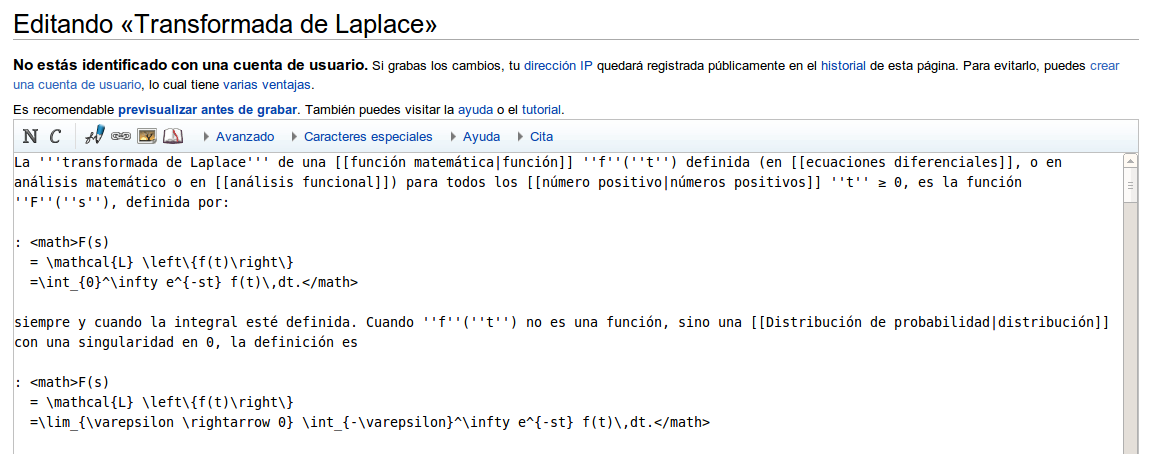
\includegraphics[width=6in]{fig/wiki_markup}
  \caption{Lenguaje Wiki Markup}
  \label{fig:wiki_markup}

\end{figure}


En los últimos años han aparecido en Internet diversos editores WYSIWYG que permiten al usuario modificar de forma inconsciente y en tiempo real el HTML del texto que introducen. Estos editores se sustentan en tecnologías como lenguajes interpretados en el lado del cliente, que ejecutados en un navegador, permiten modificar de forma dinámica el HTML del cuerpo del texto. Si esto es así, ¿por qué se siguen usando lenguajes de etiquetado intermedio?. 

El problema de permitir al usuario introducir directamente código HTML, para ser renderizado posteriormente en la página, presenta un grave riesgo para la seguridad del sistema, es por eso que en un principio se adoptaron lenguajes como BBCode para evitar este tipo de ataques. A este tipo de ataques se les conoce como amenazas XSS, y hacen referencia habitualmente a la inyección de código malicioso en el código de la página.

El trabajo de limpieza del código HTML debe ser exhaustivo, lo que hace de esta una tarea tediosa, por lo que se adoptó el camino fácil del uso de lenguajes intermedios. Es de suma importancia que el análisis del HTML generado en busca de amenazas sea efectivo y se realice de forma correcta, y dada la complejidad de dicha tarea, implementarlo nosotros mismos dentro del marco temporal de este proyecto no es una opción. En lugar de eso existen diversas alternativas en la Web que podemos usar, habiéndonos decantado finalmente por HTMLpurifier~\cite{htmlpurifier}.

El editor resultante es ligero, elegante, fácil de usar y cumple con los requisitos de edición requeridos por la plataforma SWAD. SWADE no busca la potencia de edición de otras alternativas Web como CKEditor~\cite{CKEditor:ckeditor} (al nivel de programas de ofimática como Word), para este tipo de tareas se usarán hojas de estilos CSS. En la figura ~\ref{fig:test1} podemos ver cómo queda el editor integrado en SWAD en la sección mensajes.

\begin{figure}[h!]
  \centering
      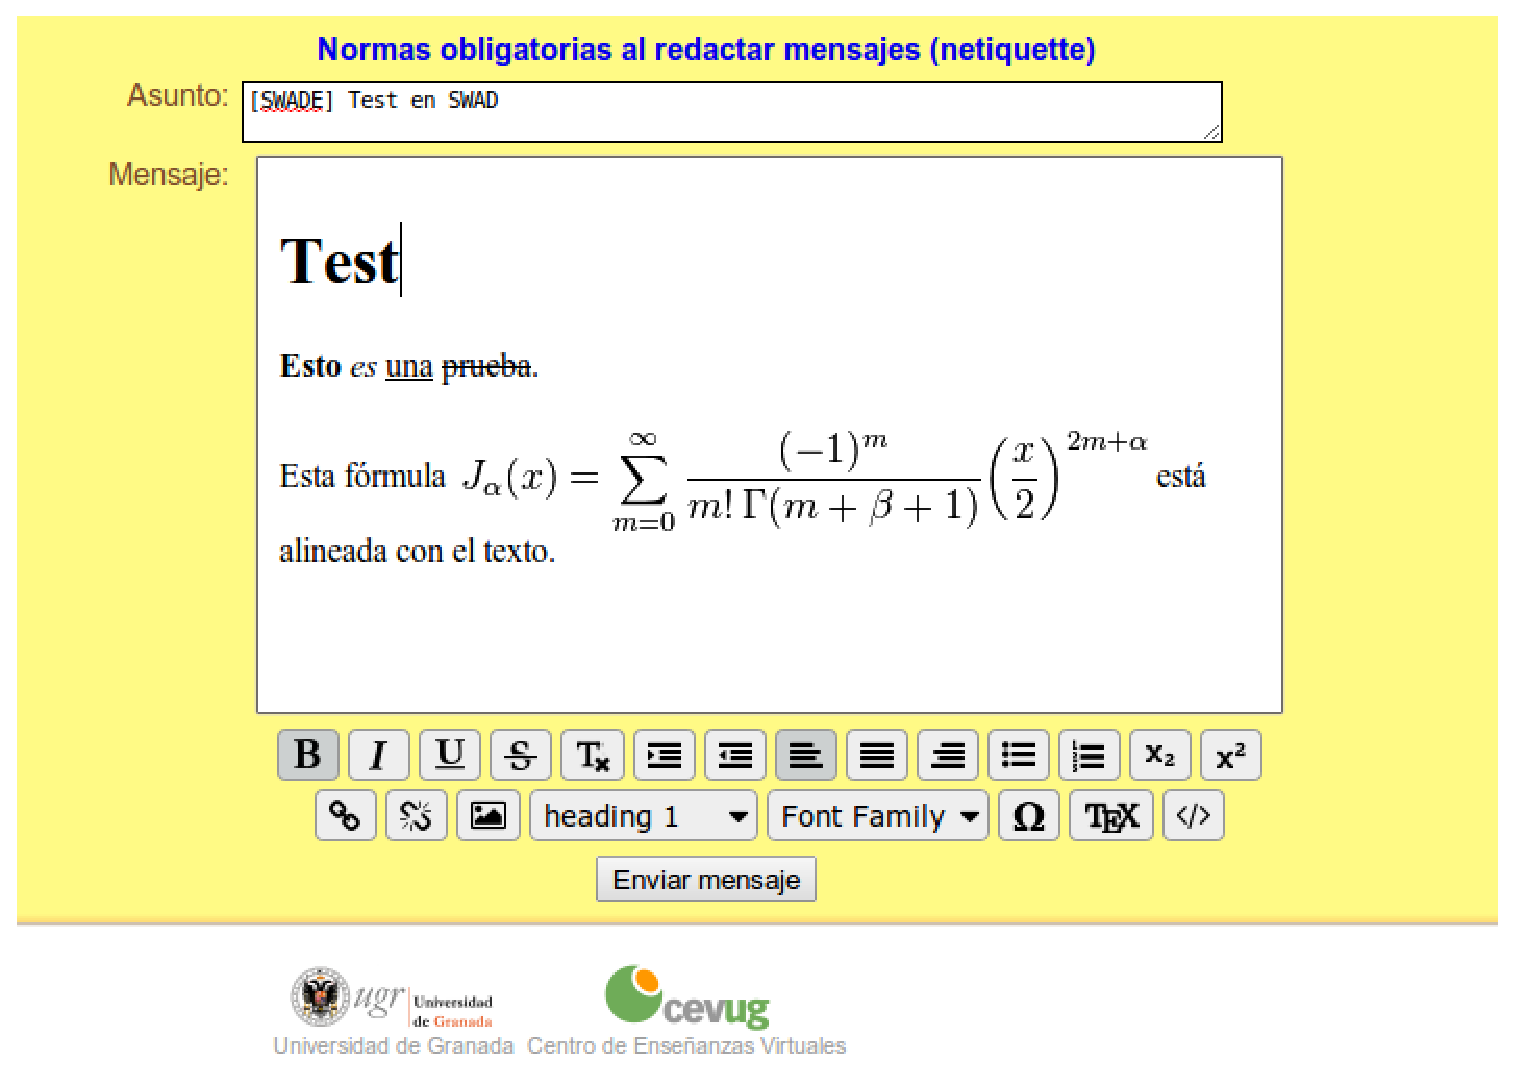
\includegraphics[width=5in]{fig/swade_test1}
  \caption{SWADE en mensajes}
  \label{fig:test1}

\end{figure}


Otra funcionalidad de la que SWAD carece es un editor de fórmulas, de gran importancia cuando se trata de introducir preguntas de tipo test. En este caso nos decantaremos por un editor sencillo basado en LaTeX, que hará indispensable que el usuario tenga unas nociones básicas de dicho lenguaje. En nuestro editor de fórmulas el usuario podrá ver mientras escribe la fórmula que se está formando. Para llevar a cabo esta tarea usamos la herramienta MathJax, que se sustenta en AJAX (Asynchronous Javascript And XML) y hace un renderizado con HTML y CSS de dicha fórmula. Este proceso se realiza en el lado del cliente (navegador web).En la figura ~\ref{fig:test2} podemos ver el editor de fórmulas.


\begin{figure}[h!]
  \centering
      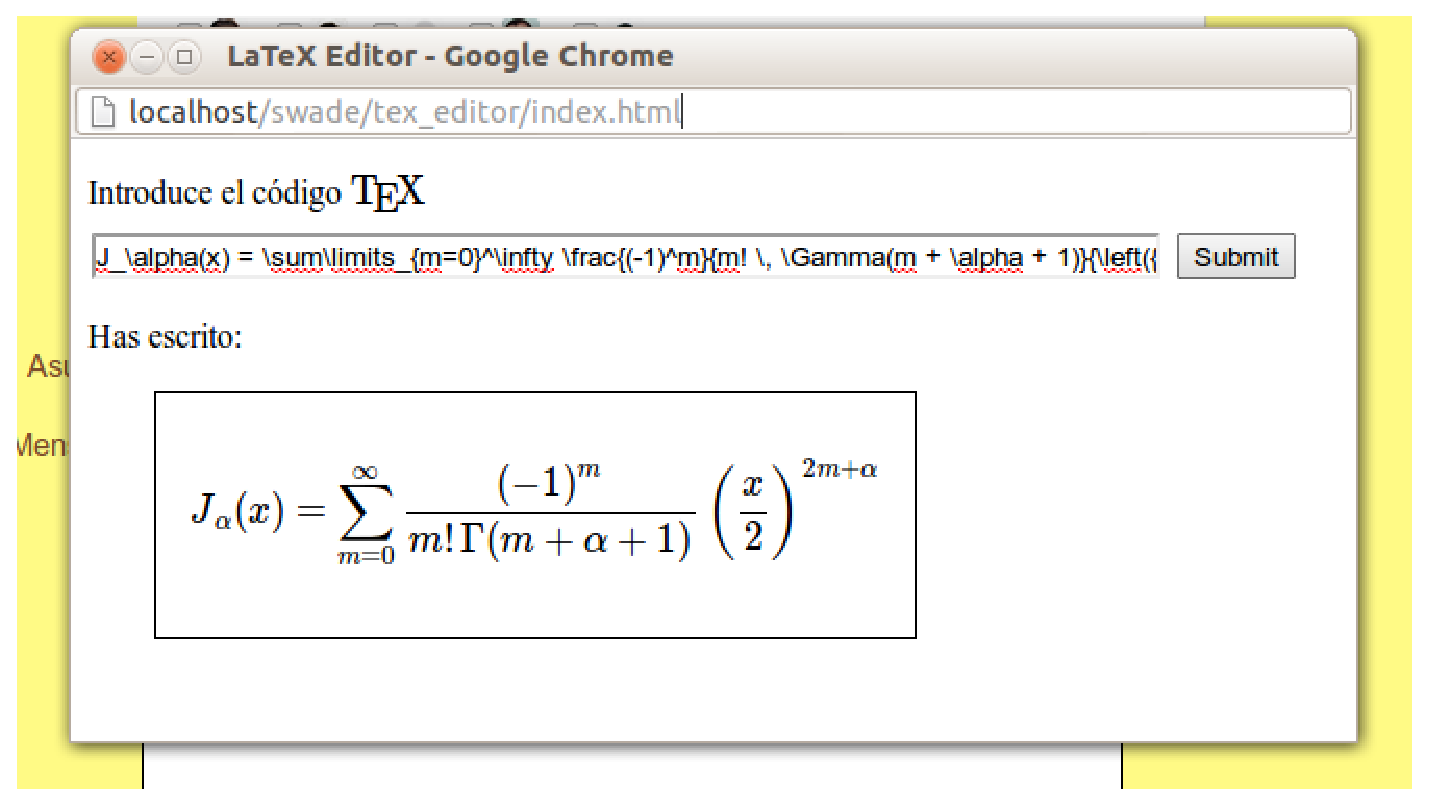
\includegraphics[width=5in]{fig/swade_test2}
  \caption{\rm\TeX\ Editor}
  \label{fig:test2}

\end{figure}

Una vez introducido el código, el usuario confirmará que es la fórmula que quiere enviándose una petición al servidor donde se generará la imagen png correspondiente a la fórmula, usando para esta tarea la herramienta texvc~\cite{texvc}, y devolviéndose finalmente el código HTML necesario para insertar dicha imagen. Esta petición al servidor se realiza de forma asíncrona usando AJAX, de forma que cuando se recibe la respuesta, el editor de fórmulas inserta el código de la imagen en el editor SWADE. 

Se ha tenido en cuenta la posibilidad de edición de una fórmula, por lo que al hacer click en una se nos abrirá el editor de fórmulas permitiéndonos ``editar'' la fórmula. Hay que decir que la imagen no se edita, como era de esperar, sino que se elimina la imagen anterior y se posiciona en su lugar una nueva imagen generada.

 


\chapter{Análisis}

El proyecto surge  a raíz de la necesidad de SWAD de un editor integrado, que permita el formato de los textos. SWAD es una plataforma muy completa en lo que a gestión docente se refiere, pero si hay un punto débil en esta es la incapacidad de un usuario de dar formato al contenido que genera o lo que es incluso más importante, insertar fórmulas matemáticas. 

\section{Requisitos funcionales}

Los requisitos de nuestro editor son los siguientes:

\begin{itemize}
\item \textbf{Simplicidad} en su uso. El usuario deberá ser capaz de usar el editor sin una fase de entrenamiento previa, cometiendo como máximo un error por cada veinte minutos de uso. 

Dado que SWAD es una plataforma usada por muchos profesores y alumnos de muy diversas titulaciones el editor debe ser lo mas simple e intuitivo posible, evitando en la representación del contenido notación HTML, bbcode o similares. Estos editores son los que se conoce como editores WYSIWYG (What You See Is What You Get).

\item Fácil \textbf{integración} con SWAD. La integración del editor en la plataforma no requerirá más de tres líneas en el código de la plataforma. Nuestro editor debe ser lo mas independiente de SWAD posible, integrándose él mismo en el código de la página HTML. 

\item Soporte para \textbf{fórmulas} matemáticas. Nuestro editor permitirá insertar fórmulas matemáticas. Además, se contemplará la posibilidad de visualización de una página con múltiples fórmulas matemáticas sin que se produzca un deterioro excesivo del rendimiento (Tiempo de carga medio de 10 fórmulas inferior a 1 segundo).

\item Inserción de \textbf{símbolos}. Nuestro editor permitirá la inserción de símbolos tales como letras griegas y operadores matemáticos y algebraicos.

\item Posibilidad de ver y editar el \textbf{código HTML} generado, así como generar un código HTML de calidad, controlando etiquetas no cerradas y bloqueando etiquetas no permitidas para que el contenido global de la página no se vea afectado y evitar ataques XSS respectivamente.

\item \textbf{Formato simple de texto} y su estructura. Principalmente negrita, cursiva, subrayado, tachado y viñetas, subíndices, superíndices así como formato de cabeceras y cuerpo de texto y tipos de letra normal y mono-espaciada. 

\item El editor permitirá añadir \textbf{imágenes} y \textbf{enlaces}.

\item \textbf{Disponibilidad} del servicio. Por eso no debemos usar ninguna herramienta online, ya que no tenemos ninguna garantía de la continuidad de estos servicios. Por el mismo motivo usaremos tecnologías poco susceptibles de cambio, para reducir de esta manera las posibles labores de mantenimiento.

\item \textbf{Seguridad}. Permitir al usuario modificar directamente el HTML de la página conlleva un grave riesgo para la seguridad del sistema. Por ello, debemos filtrar el HTML generado con el fin de evitar las amenazas de inyección de código malicioso (XSS) en la plataforma.

\end{itemize}

\section{Visión global de la solución}
De lo anteriormente expuesto, podemos extraer que en el lado del cliente (Navegador Web) se dará formato al texto que introducimos, mientras que en el lado del servidor nos ocuparemos de generar las imágenes de las fórmulas y limpiar el código HTML generado.

Generando las imágenes de las fórmulas en el servidor nos aseguramos de que se cumple el requisito de tiempo impuesto a la carga de imágenes. Aunque puede producirse un pequeño deterioro en el rendimiento al cargar las imágenes, esto ocurrirá solo la primera vez ya que la caché del navegador hará que la carga las veces posteriores sea imperceptible. 

\section{Integración en la Plataforma}

En esta sección analizaremos las distintas partes de la plataforma SWAD en las que es necesario el uso del editor SWADE. Es importante un análisis de los lugares de la plataforma en los que se insertará el editor para que el diseño de la solución se adapte de la forma mas simple y elegante posible a cada caso.

Usaremos el editor SWADE para introducir la información de las distintas asignaturas. Dados de alta como profesores, en la pestaña Asignatura, debemos usar el editor en las secciones Introducción, Guía docente, Programa teoría, Programa prácticas,  Bibliografía, FAQ, Enlaces y en la pestaña Evaluación a la sección Sistema de Evaluación. En la figura ~\ref{fig:asig} podemos ver las distintas secciones donde vamos a integrar el editor.


\begin{figure}
        \centering
        \begin{subfigure}[b]{0.3\textwidth}
                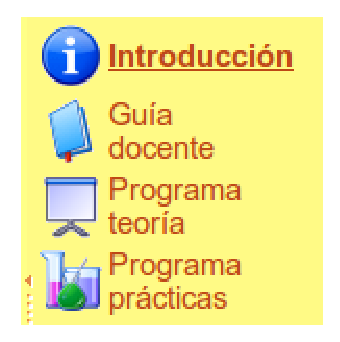
\includegraphics[width=\textwidth]{fig/inte_asig1}
                %\caption{A gull}
                \label{fig:inte_asig1}
        \end{subfigure}%
        ~ %add desired spacing between images, e. g. ~, \quad, \qquad etc.
          %(or a blank line to force the subfigure onto a new line)
        \begin{subfigure}[b]{0.3\textwidth}
                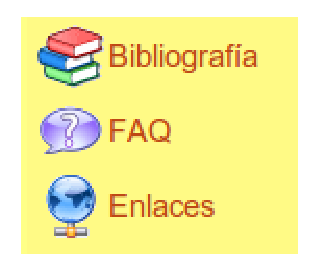
\includegraphics[width=\textwidth]{fig/inte_asig2}
                %\caption{A tiger}
                \label{fig:inte_asig2}
        \end{subfigure}
        ~ %add desired spacing between images, e. g. ~, \quad, \qquad etc.
          %(or a blank line to force the subfigure onto a new line)
        \begin{subfigure}[b]{0.3\textwidth}
                
\includegraphics[width=\textwidth]{fig/inte_eva}
                %\caption{A mouse}
                \label{fig:inte_eva}
        \end{subfigure}
        \caption{Secciones de info. asignaturas donde vamos a integrar SWADE }\label{fig:asig}
\end{figure}


En todas estas opciones, en el menú de edición, se nos preguntará el método por el que vamos a editar dicha sección, donde podremos seleccionar nuestro editor, tal como podemos ver en la figura ~\ref{fig:inte_sel}. 
  

\begin{figure}[h!]
  \centering
      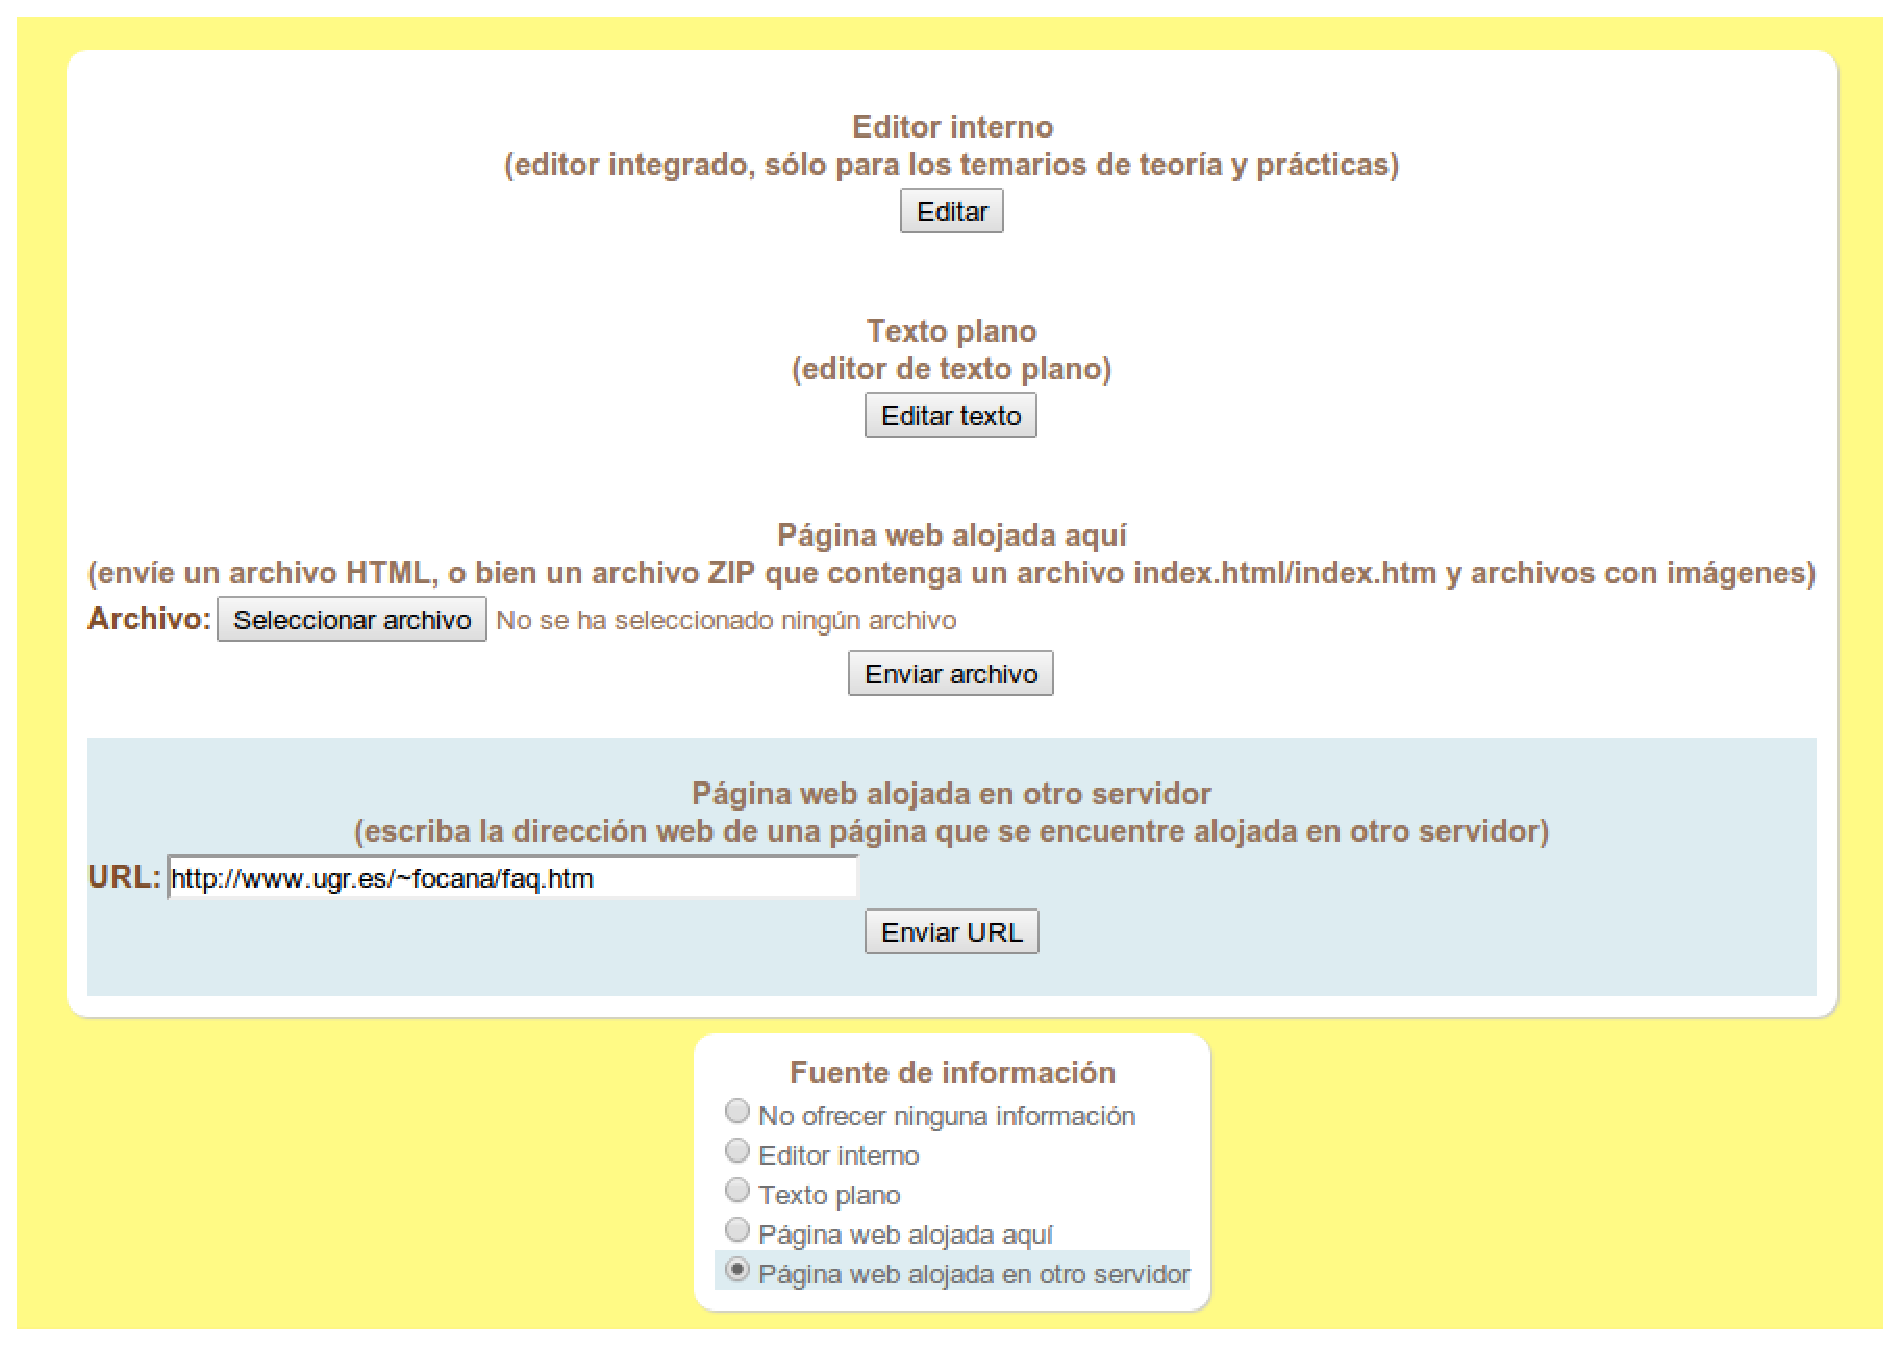
\includegraphics[width=7in]{fig/inte_sel}
  \caption{Menú de selección de método de edición.}
  \label{fig:inte_sel}

\end{figure}


También será necesario integrar SWADE en el campo descripción de Actividades y Encuestas de las pestañas Evaluación y Estadísticas respectivamente. En la figura ~\ref{fig:inte_acti} podemos ver el formulario de creación de una nueva actividad. El formulario de creación de una nueva encuesta es muy similar.

\begin{figure}[h!]
  \centering
      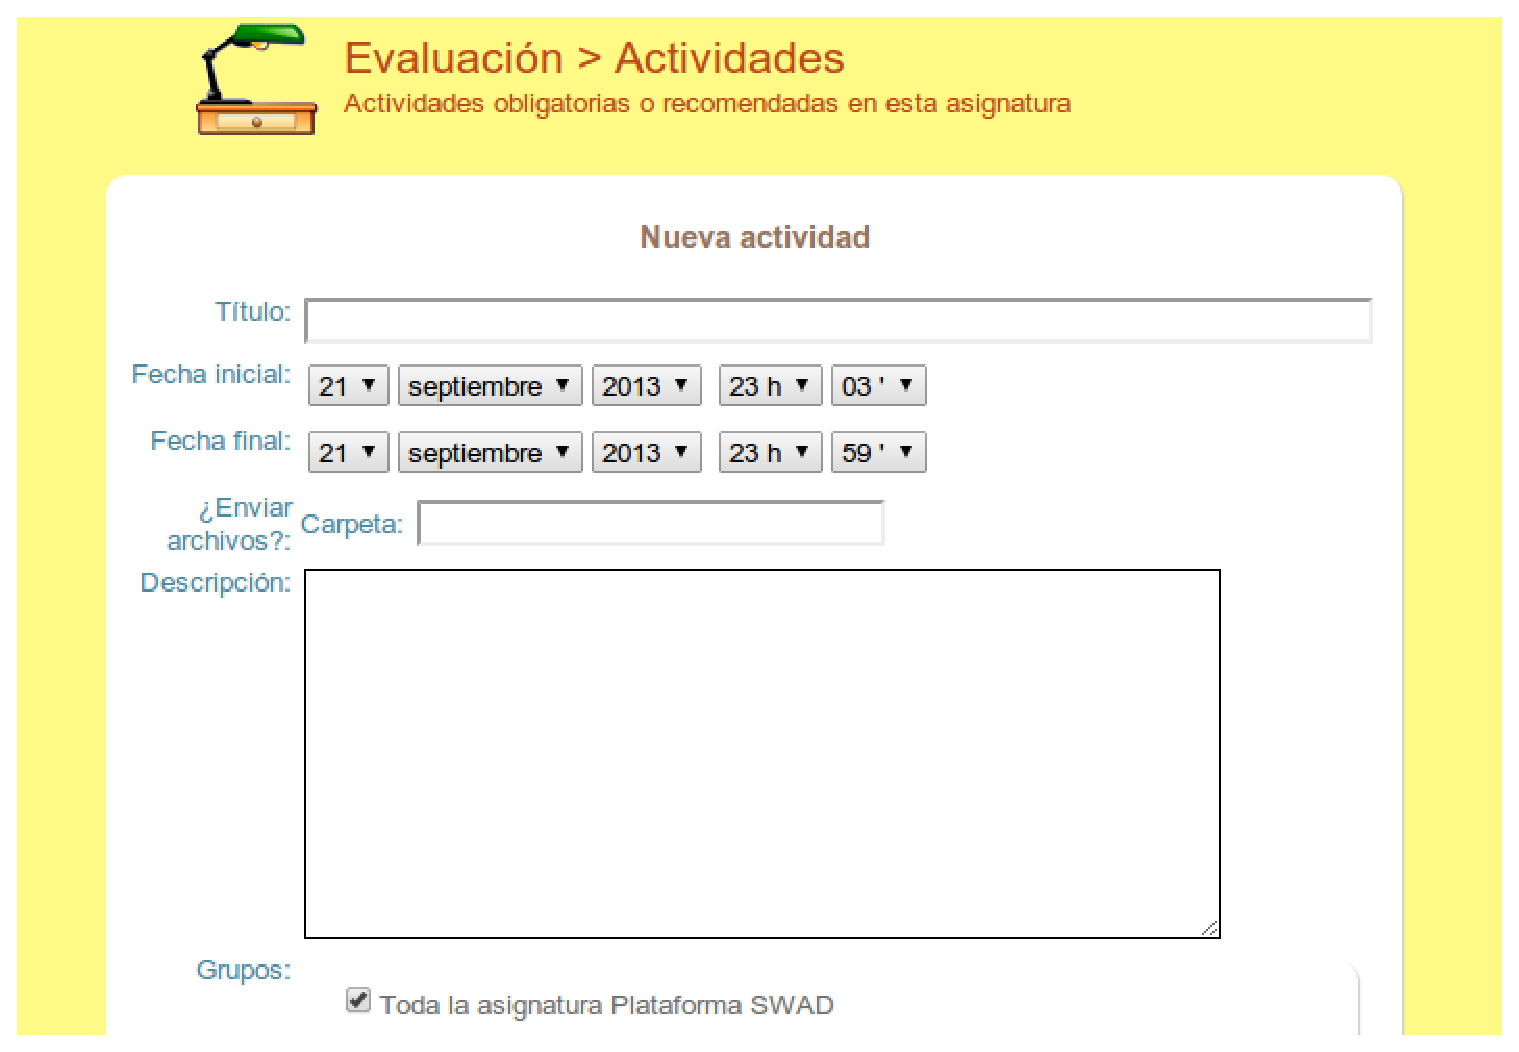
\includegraphics[width=4in]{fig/inte_acti}
  \caption{Creación de una nueva actividad.}
  \label{fig:inte_acti}

\end{figure}


Debemos contemplar también la posibilidad de creación de múltiples editores en un mismo documento HTML ya que, en la sección de Test de la pestaña Evaluación, debemos insertar un total de veintidós editores cada vez que creamos una nueva pregunta. Serían dos por cada posible respuesta, haciendo un total de veinte, más dos por el enunciado y la realimentación de este. En las figuras ~\ref{fig:inte_test1} e ~\ref{fig:inte_test2} podemos ver el formulario de creación de una nueva pregunta de test.

\begin{figure}[h!]
  \centering
      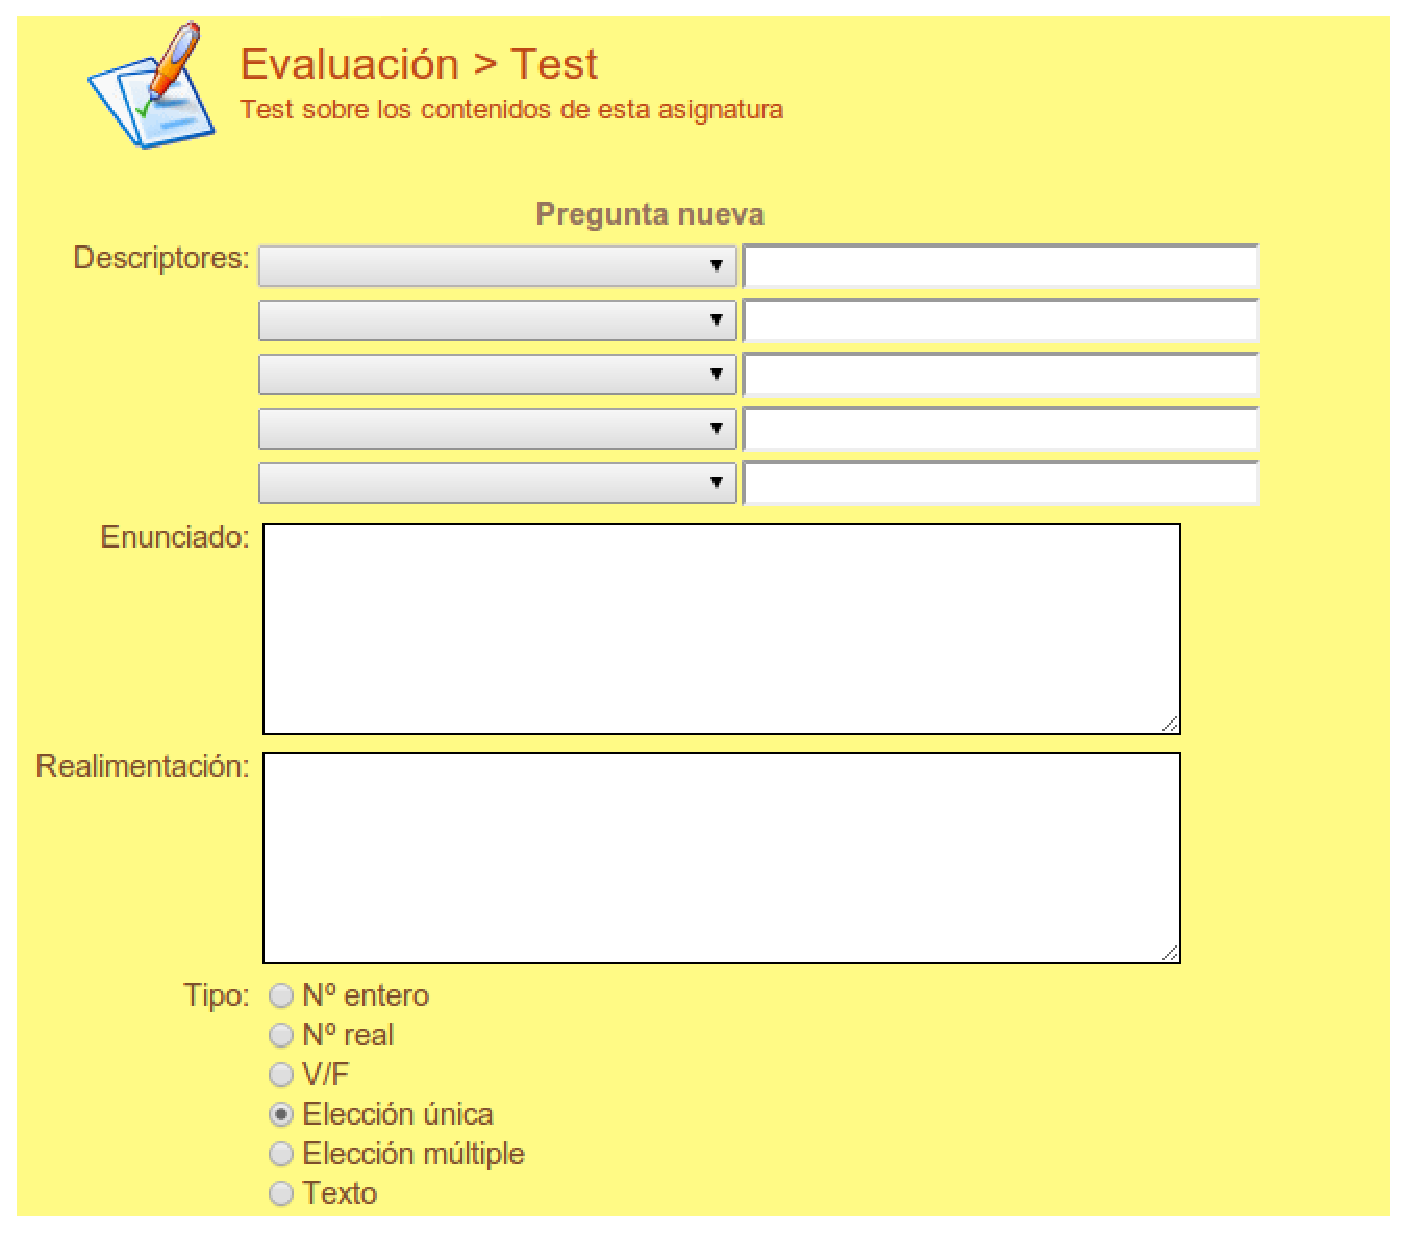
\includegraphics[width=4in]{fig/inte_test1}
  \caption{Creación de un nuevo test. Enunciado.}
  \label{fig:inte_test1}

\end{figure}

\begin{figure}[h!]
  \centering
      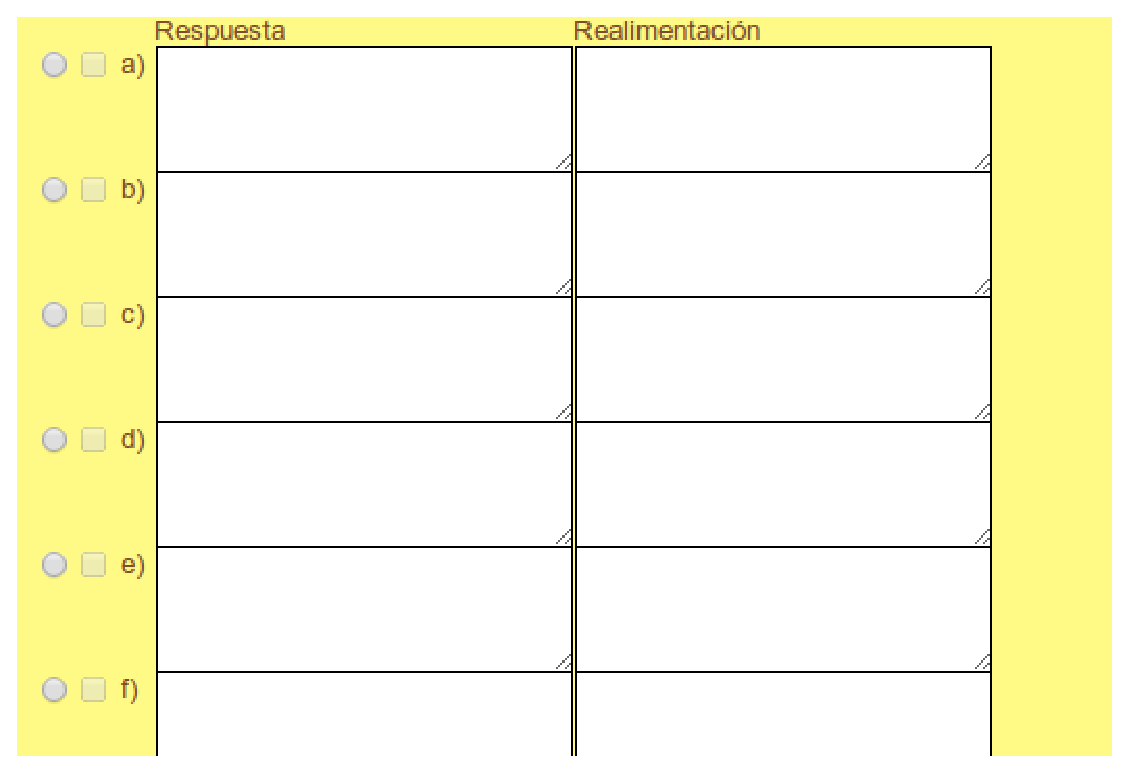
\includegraphics[width=4in]{fig/inte_test2}
  \caption{Creación de un nuevo test. Respuestas.}
  \label{fig:inte_test2}

\end{figure}


Finalmente debemos instanciar SWADE en los mensajes de SWAD, ya sea Mensajes entre usuarios o en los Foros. En principio no será necesario integrarlo en los Avisos. Tampoco es necesario en principio integrarlo en Convocatoria de examen o los Campos de las fichas. En la figura ~\ref{fig:inte_men} podemos ver donde tendremos que insertar el editor para los mensajes.

\begin{figure}[h!]
  \centering
      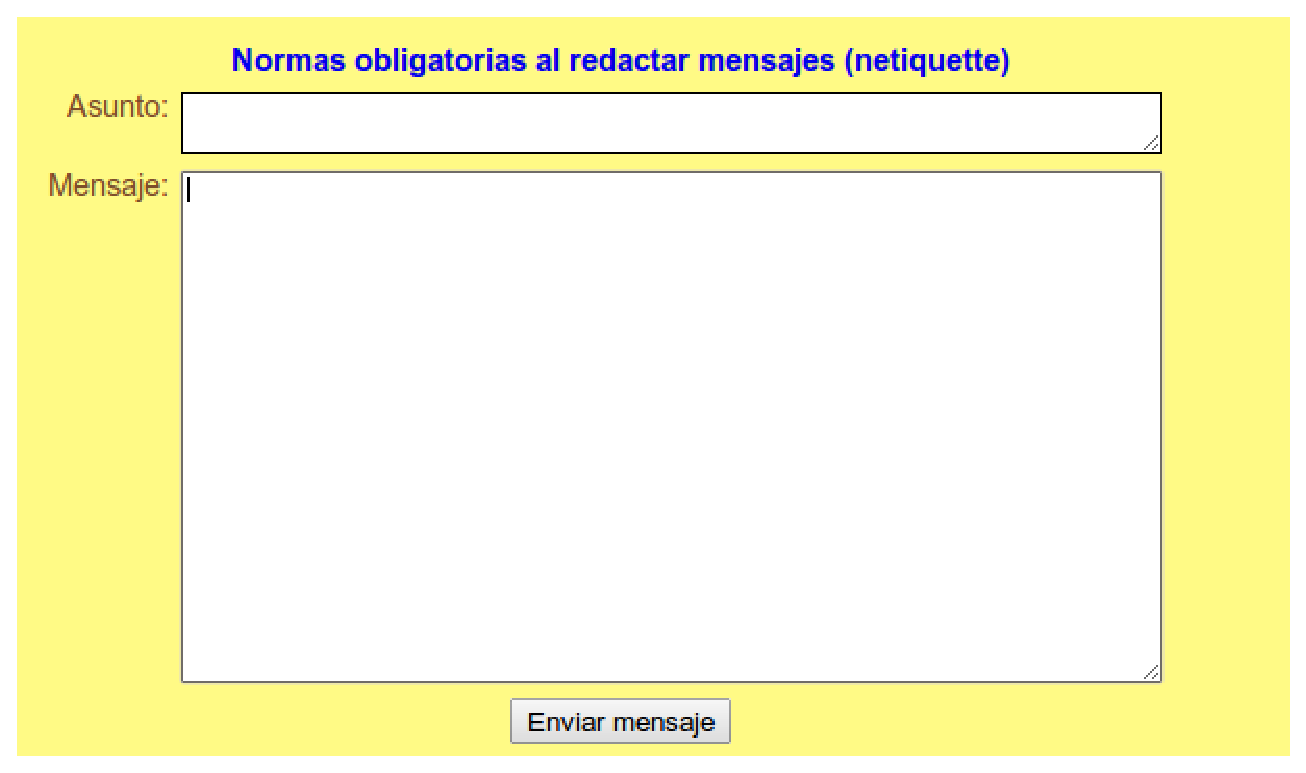
\includegraphics[width=4in]{fig/inte_men}
  \caption{Mensajes de SWAD}
  \label{fig:inte_men}

\end{figure}

%\chapter{Editor WYSIWYG}

Este capítulo es una introducción a los editores WYSIWYG. 

\section{¿Qué es un editor WYSIWYG?}

WYSIWYG es el acrónimo de What You See Is What You Get. Un editor WYSIWYG es un sistema en el cual el contenido (texto y graficos) mostrado en pantalla durante la edición aparece de igual forma a la forma en la que se muestra, la cual puede ser un documento, una página web o una presentación.

\section{Funcionamiento de un editor WYSIWYG}


\section{HTML5 y editores WYSIWYG}


\section{Implementando un editor WYSIWYG}



\chapter{Estado del arte}
En todo proceso de investigación y desarrollo de software, es importante dedicar un tiempo a examinar en que punto se encuentra la investigación en dicho campo. Por tanto, antes de empezar a diseñar nuestra solución nos dedicaremos al análisis de diversas plataformas y editores que resuelven problemas similares al que nos ocupa.

Dedicaremos este capítulo al análisis de diversas plataformas online y editores WYSIWYG. Nos centraremos principalmente en Wikipedia, Stackoverflow y algunos editores como YUI Rich Text Editor~\cite{YUIEditor:yuieditor}, NicEdit~\cite{NicEdit:nicedit}, CKEditor~\cite{CKEditor:ckeditor}, TinyMCE~\cite{TinyMCE:tinymce} y openWYSIWYG~\cite{openWYSIWYG:openwysiwyg}.

\section{Plataformas}
\subsection{Wikipedia}

Wikipedia usa un editor WYSIWYM (What You See IS What You Mean) bastante simple, usando solo las características que la plataforma necesita. Este tipo de editores se caracteriza por una total separación entre la presentación y el contenido del texto. Para el etiquetado usa un lenguaje propio llamado Wiki markup. En la figura ~\ref{fig:wiki_wysiwym} podemos ver el aspecto del editor de Wikipedia.

Como inconvenientes de este tipo de editores podemos destacar la complejidad en su uso. Tal y como dijimos anteriormente la plataforma SWAD es usada por alumnos y profesores de gran variedad de titulaciones, por lo que uno de los requisitos es la facilidad de uso, es por eso por lo nos decantamos por un editor del tipo WYSIWYG (What You See Is What You Get), donde el usuario ``obtiene lo que ve'', manipulando, de forma directa e inconsciente, el código HTML del contenido que genera, sin un lenguaje de etiquetado intermedio. 

\begin{figure}[h!]
  \centering
      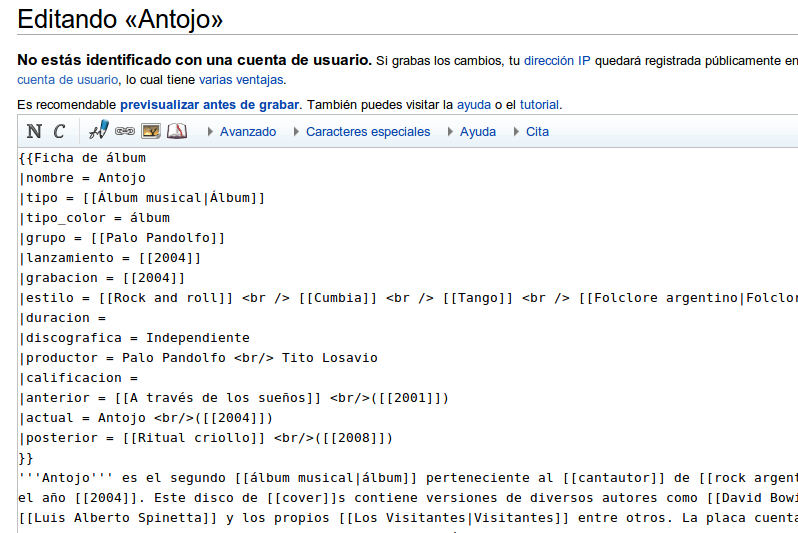
\includegraphics[width=1.0\textwidth]{fig/wiki_wysiwym}
  \caption{Editor WYSIWYM de Wikipedia}
  \label{fig:wiki_wysiwym}
\end{figure}

En la actualidad se está implantando en Wikipedia un editor WYSIWYG el cual se encuentra en fase beta y aún no soporta toda la funcionalidad del editor WYSIWYM, como por ejemplo la inserción de fórmulas matemáticas. En la figura ~\ref{fig:wiki_wysiwyg} podemos ver el aspecto de dicho editor, editando el mismo artículo que en la figura ~\ref{fig:wiki_wysiwym}.

\begin{figure}[h!]
  \centering
      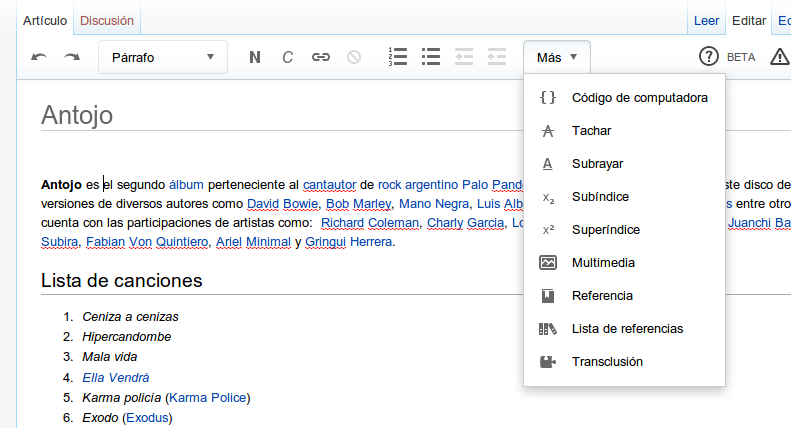
\includegraphics[width=1.0\textwidth]{fig/wiki_wysiwyg}
  \caption{Editor WYSIWYG de Wikipedia}
  \label{fig:wiki_wysiwyg}
\end{figure}

Sin embargo lo que nos interesa de Wikipedia, más que el editor en sí, es la capacidad de este para la inserción de fórmulas en {\LaTeX}~\cite{wikiform}.

MediaWiki usa un subconjunto del etiquetado AMS-LaTeX, que a su vez es un superconjunto de {\LaTeX} y presenta dos opciones para trabajar con fórmulas. La primera consiste en la generación de imágenes PNG a partir de las fórmulas usando Texvc~\cite{texvc} y la segunda que renderiza las ecuaciones mediante CSS y HTML usando MathJax~\cite{mathjax}.

Visualmente, MathJax proporciona mejores resultados. La calidad de la tipografía es muy superior y se eliminan ciertos problemas, como el diferente tamaño de las fórmulas con respecto al texto circundante o falta de alineación. Por otro lado, la herramienta javascript empleada por MathJax para interpretar las expresiones matemáticas toma más tiempo que Texvc.

Otra de las ventajas del uso de imágenes png en lugar de renderizar fórmulas con HTML y CSS es que las imágenes podrán ser almacenadas en cache, permitiendo que futuros accesos a la página sean mas rápidos.

Por otra parte, el uso de Texvc presenta el problema del tamaño de las fórmulas.
 
\subsection{Stackoverflow}
La web Stackoverflow usa un editor WYSIWYM, al estilo del que usa Wikipedia, que combina un lenguaje de etiquetado intermedio con un subconjunto del lenguaje de etiquetado HTML. Este editor posee un campo que muestra, al mismo tiempo que editamos, el resultado final del contenido que generamos. Además, tal cómo se muestra en la figura ~\ref{fig:stack_editor}, posee un menú de ayuda desplegable que permite consultarlo de forma muy cómoda mientras se escribe. Estos dos aspectos hacen que este editor sea mucho mas sencillo de usar que el editor WYSIWYM que posee Wikipedia, aunque, todo sea dicho, el editor de Wikipedia contempla funcionalidad, como el soporte de fórmulas LaTeX entre otros, que este no posee. 

\begin{figure}[h!]
  \centering
      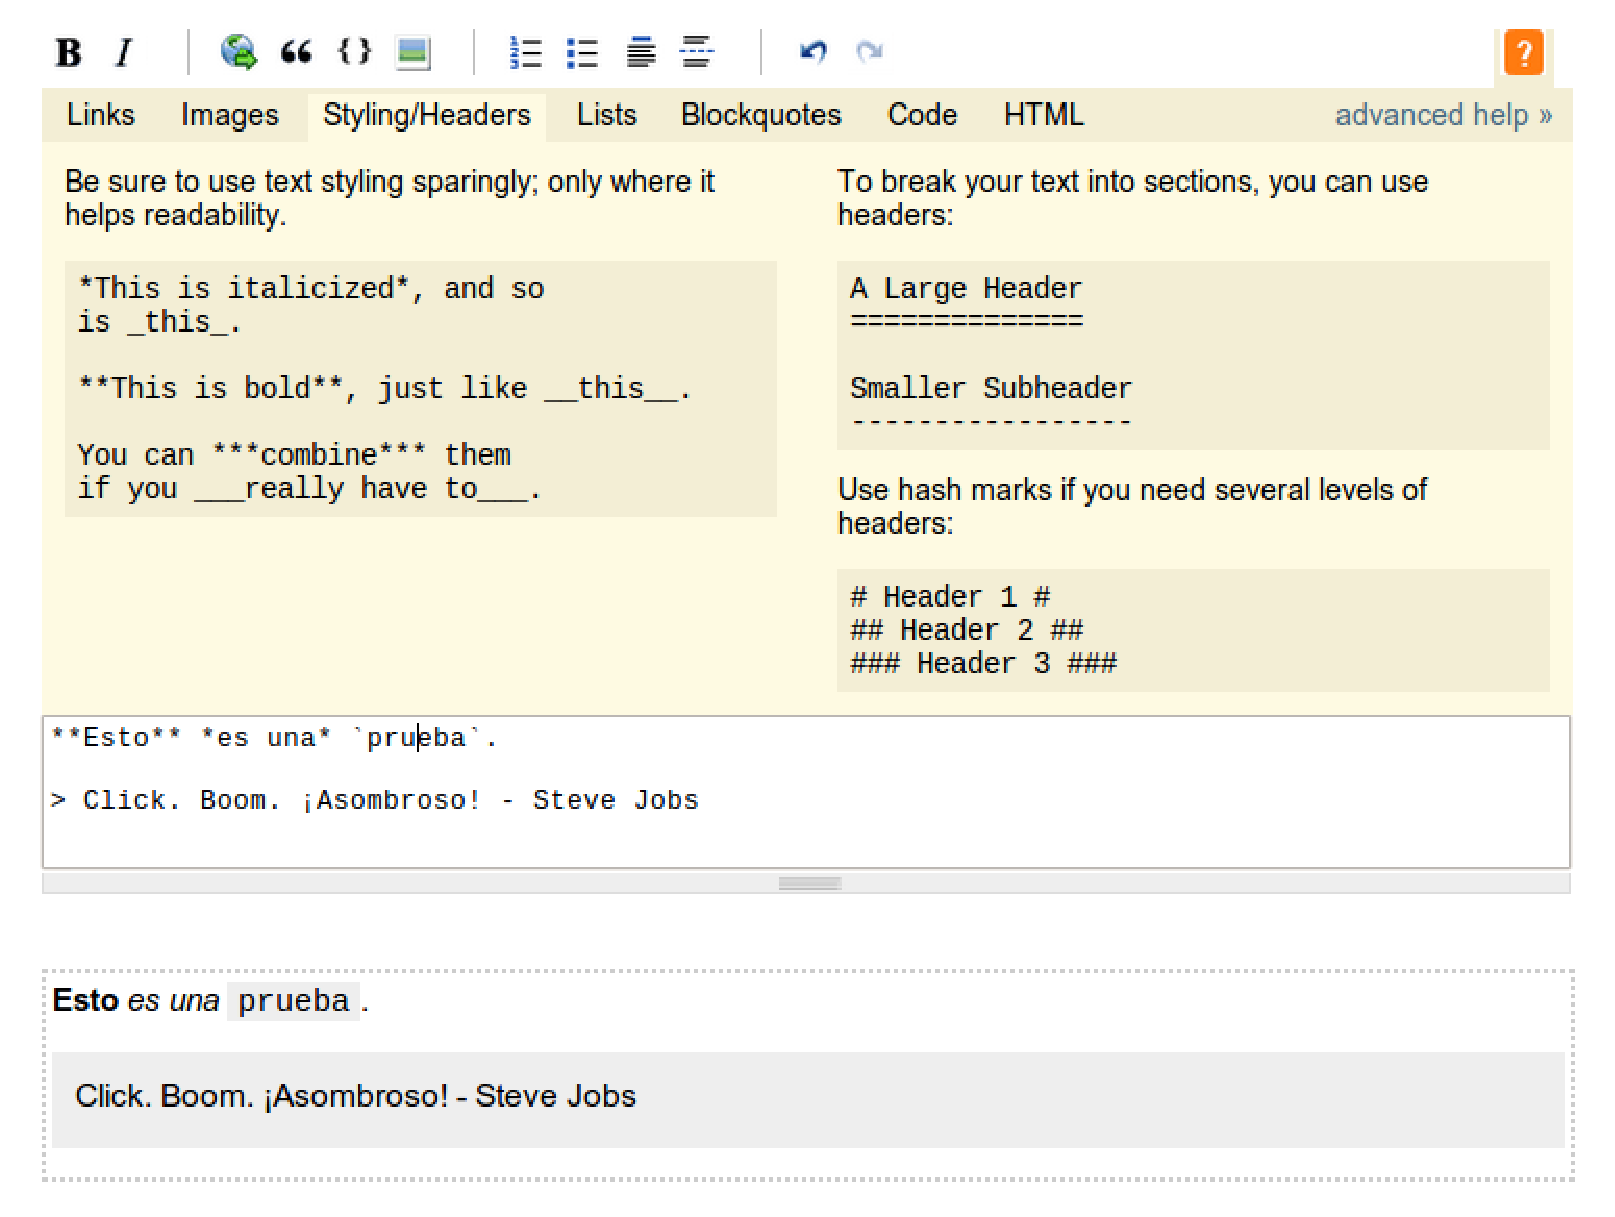
\includegraphics[width=1.0\textwidth]{fig/stack_editor}
  \caption{Editor WYSIWYM de Stackoverflow}
  \label{fig:stack_editor}
\end{figure}

\section{Renderizado de Fórmulas}
\subsection{MathJax}

MathJax, tal y como se define en su página, es un motor de visualización JavaScript para fórmulas matemáticas y de código abierto que funciona en todos los navegadores. Dicha aplicación, como ya hemos comentado previamente, nos permite renderizar las fórmulas {\LaTeX} mediante HTML y CSS.

MathJax analiza el contenido de la página buscando una fórmula en {\LaTeX} y cuando la encuentra la sustituye por un conjunto de etiquetas que compondrán la fórmula renderizada.

Esta herramienta permite dos modos de uso. La primera es enlazando directamente la aplicación a través de la Red de Distribución de Contenido (CDN) de MathJax. De esta forma MathJax siempre estará actualizado y además te ahorras su instalación en el servidor.

Sin embargo, tal cómo dijimos antes, buscamos herramientas instalables en el servidor, ya que no podemos estar sujetos a la disponibilidad de servicios de terceros. Por este motivo, si nos decantamos a usar MathJax, optaremos por la descarga e instalación de MathJax en el servidor.

\subsection{Texvc}

Texvc (Tex validator and converter) es la herramienta usada por Wikipedia para validar y generar imágenes png a partir del código en formato ams-latex. 

Dicha herramienta tiene una serie de dependencias que tendremos que satisfacer. Estas dependencias son ocaml, el lenguaje en la que está implementada y latex, dvips, gs y convert, usadas en el proceso de renderizado de la imagen de la fórmula.

A pesar de la escasa documentación disponible de esta herramienta, su extendido uso ha dado lugar a un completo FAQ con problemas de uso y soluciones para dichos problemas. El motivo por el que dicha herramienta se usa tanto es porque pertenece a la extensión math de mediawiki.

\subsection{tex2png}

Tex2png es una herramienta simple que cumple perfectamente con nuestro propósito. El autor la describe en su página~\cite{xyne:tex2png} como una herramienta para pasar fácilmente del formato {\TeX} y {\LaTeX} a PNG. Es un simple envoltorio  de \emph{latex} y \emph{divpng} que fue originalmente escrito como \emph{backend} de la web donde se aloja para insertar fácilmente fórmulas matemáticas. 

Tex2png es un script bash, por lo que su instalación consistirá únicamente en copiarlo a la carpeta desde donde lo vamos a llamar (y en la instalación de \emph{latex} y \emph{divpng}).

La documentación de esta herramienta es bastante escasa y se han encontrado algunos problemas de renderizado con algunas fórmulas. 

\section{Editores WYSIWYG}

Hay muchas personas muy inteligentes que ya han dedicado mucho tiempo a trabajar en este tema, pero esto no quiere decir que todo esté hecho. Debemos plantearnos cómo podemos mejorar estas soluciones. Obviamente, el concepto ``mejorar'' es muy difuso, puede significar que algo funcione más rápido, de una forma más novedosa o que sea más barato que el sistema original. En nuestro caso es tremendamente importante que se integre a la perfección con la plataforma SWAD y que cumpla una serie de requisitos muy concretos. En esta sección analizaremos las características de los editores WYSIWYG más usados en la Web, así como los puntos a favor y en contra de cada uno. 

También tendremos en mente las licencias bajo las que se distribuyen, pues en caso de usar parte de algún editor en nuestra solución, su licencia debe ser compatible con la licencia Affero GPL de SWAD. En la sección Apéndices podemos consultar las características generales de las distintas licencias. En caso de querer ampliar dicha información, podemos acudir a la Bibliografía.

\subsection{YUI Rich Text Editor}

Basado en la librería YUI de Yahoo y liberado bajo licencia ~\cite{BSD:bsd}, este editor sustituye el textarea estándar de HTML por un editor bastante completo. Permite dar un formato de texto enriquecido, incluyendo elementos para modificar la estructura del texto como listas, elementos para dar formato e inclusión de imágenes drag-and-drop y redimensionado de estas. Permite soporte para plugins y tiene dos modos, normal y simple, el cual tiene con un conjunto de características más reducido.

Podemos decir que se trata de un editor de alta complejidad, que se apoya en un completo Framework como es la la librería YUI de Yahoo. La Web de este editor es \url{http://yuilibrary.com/yui/docs/editor/} y allí podremos encontrar gran cantidad de información y una amplia documentación tanto de este como del Framework en el que se apoya. 

\begin{figure}[h!]
  \centering
      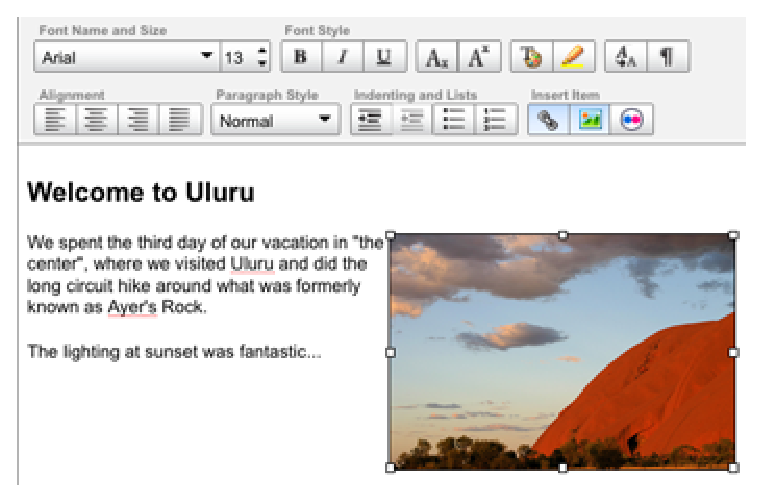
\includegraphics[width=1.0\textwidth]{fig/yuie1}
  \caption{YUI Editor}
\end{figure}

\subsection{TinyMCE}

 Este popular editor WYSIWYG transforma nuestro tradicional textarea por un conjunto de elementos HTML para construir el menú de formato, esta herramienta es muy usada por diversos CMS (Content Management System ) Open Source, es muy fácil de integrar, permite la personalización de botones en la barra de herramientas y tiene opciones para configurar el menú de formato limitando el número de botones que aparecen. Como ventaja comentar que se distribuye bajo la licencia de código abierto LGPL~\cite{LGPL:lgpl} y que es fácil de integrar y personalizar. Para probar este editor o ampliar esta información se recomienda consultar la web \url{http://www.tinymce.com/}.

\begin{figure}[h!]
  \centering
      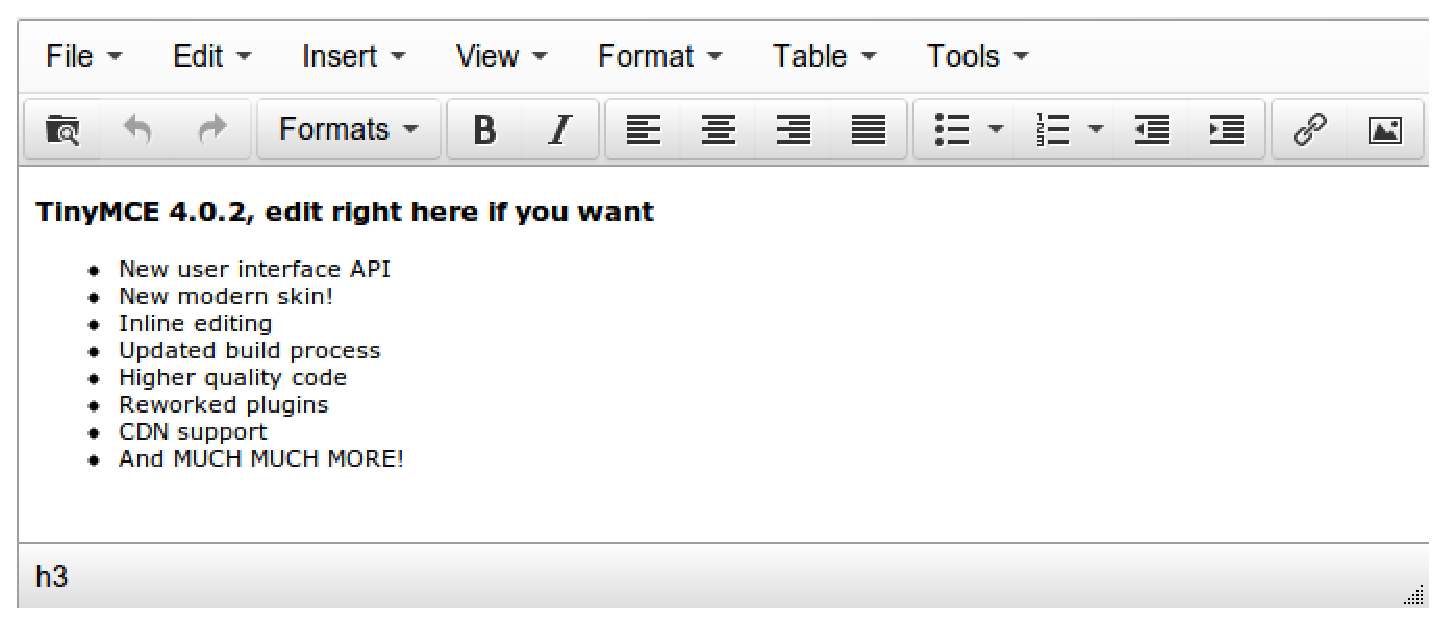
\includegraphics[width=1.0\textwidth]{fig/tmce1}
  \caption{Tinymce Editor}
\end{figure}

\subsection{NicEdit}

Este ligero editor WYSIWYG, distribuido bajo Licencia MIT~\cite{MITL:mitl}, se caracteriza por su flexibilidad, sencillez y capacidad de personalización. Permite transformar cualquier elemento div o textarea en un editor de texto enriquecido. Se trata de un editor simple pero efectivo. Al contrario que otros editores, no viene con distintos skins o plugins para ampliar su funcionalidad, ni tiene soporte nativo para fórmulas. 

Permite limitar la funcionalidad mediante la selección de los elementos que aparecerán en la barra de herramientas y, a excepción del editor de fórmulas, implementa toda la funcionalidad que requerirá nuestro editor. De fácil instalación y uso es una opción muy a tener en cuenta. La integración en la página es muy simple y puede llevarse a cabo con un par de líneas de código. Para más información visitar su web: \url{http://nicedit.com/}.


\begin{figure}[h!]
  \centering
      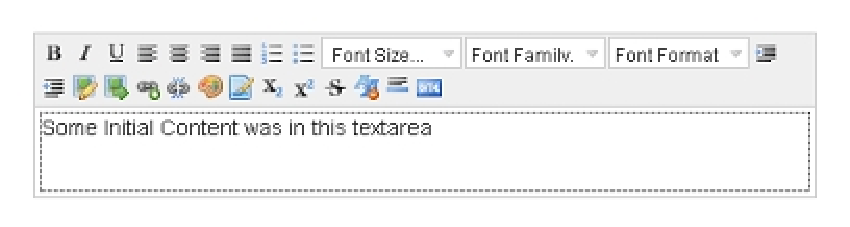
\includegraphics[width=1.0\textwidth]{fig/nice1}
  \caption{NicEdit Editor}
\end{figure}

\subsection{CKeditor}

Este editor WYSIWYG es muy potente y estable a la vez que flexible. Ampliamente usado, cuenta con una trayectoria de 10 años en el mercado. Además genera código XHTML de calidad, permitiendo su edición y parsea el contenido para que este no afecte a la página que contiene al editor. Permite el uso de plugins desarrollados por terceros y con estos amplia notablemente la funcionalidad del editor. La apariencia está muy cuidada y hay disponibles varios skins que podemos usar. Distribuido bajo las licencias de código abierto GPL~\cite{GPL:gpl}, LGPL~\cite{LGPL:lgpl} y MPL~\cite{MPL:mpl}.

Presenta la ventaja de tener soporte para fórmulas mediante plugins. Los plugins con esta finalidad disponibles son dos: Math Editor y WIRIS math \& science editor. El primero funcionaba correctamente en pruebas online, pero al probarlo en nuestro servidor no hemos conseguido que funcione en ningún navegador, muy probablemente por imcopatibilidades con la versión de CKEditor. El segundo plugin cumple con su cometido, aunque desde mi punto de vista es demasiado complejo. Tras seleccionar la opción de fórmulas, tal y como se muestra en la Figura ~\ref{fig:ckmath}, se abre una nueva ventana que contiene un completo editor donde podemos escribir nuestra fórmula. Una vez confirmada la operación se inserta en nuestro editor la imagen correspondiente a la fórmula escrita. Pese a estos pequeños fallos en los plugins, que recordemos han sido desarrollados por terceros, el editor en sí es muy completo y permite entre otras cosas la edición de texto en linea al hacer click sobre este. 

Para más información podemos consultar su web: \url{http://ckeditor.com/}

\begin{figure}[h!]
  \centering
      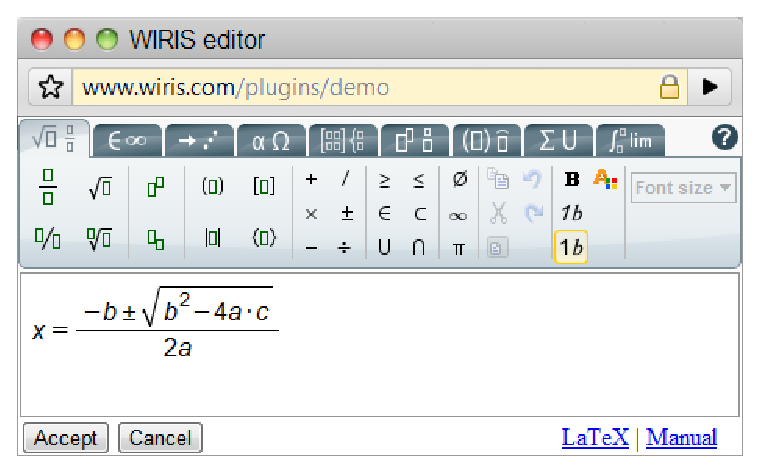
\includegraphics[width=1.0\textwidth]{fig/cke3}
  \caption{Plugin WIRIS para CKEditor}
  \label{fig:ckmath}
\end{figure}

\begin{figure}[h!]
  \centering
      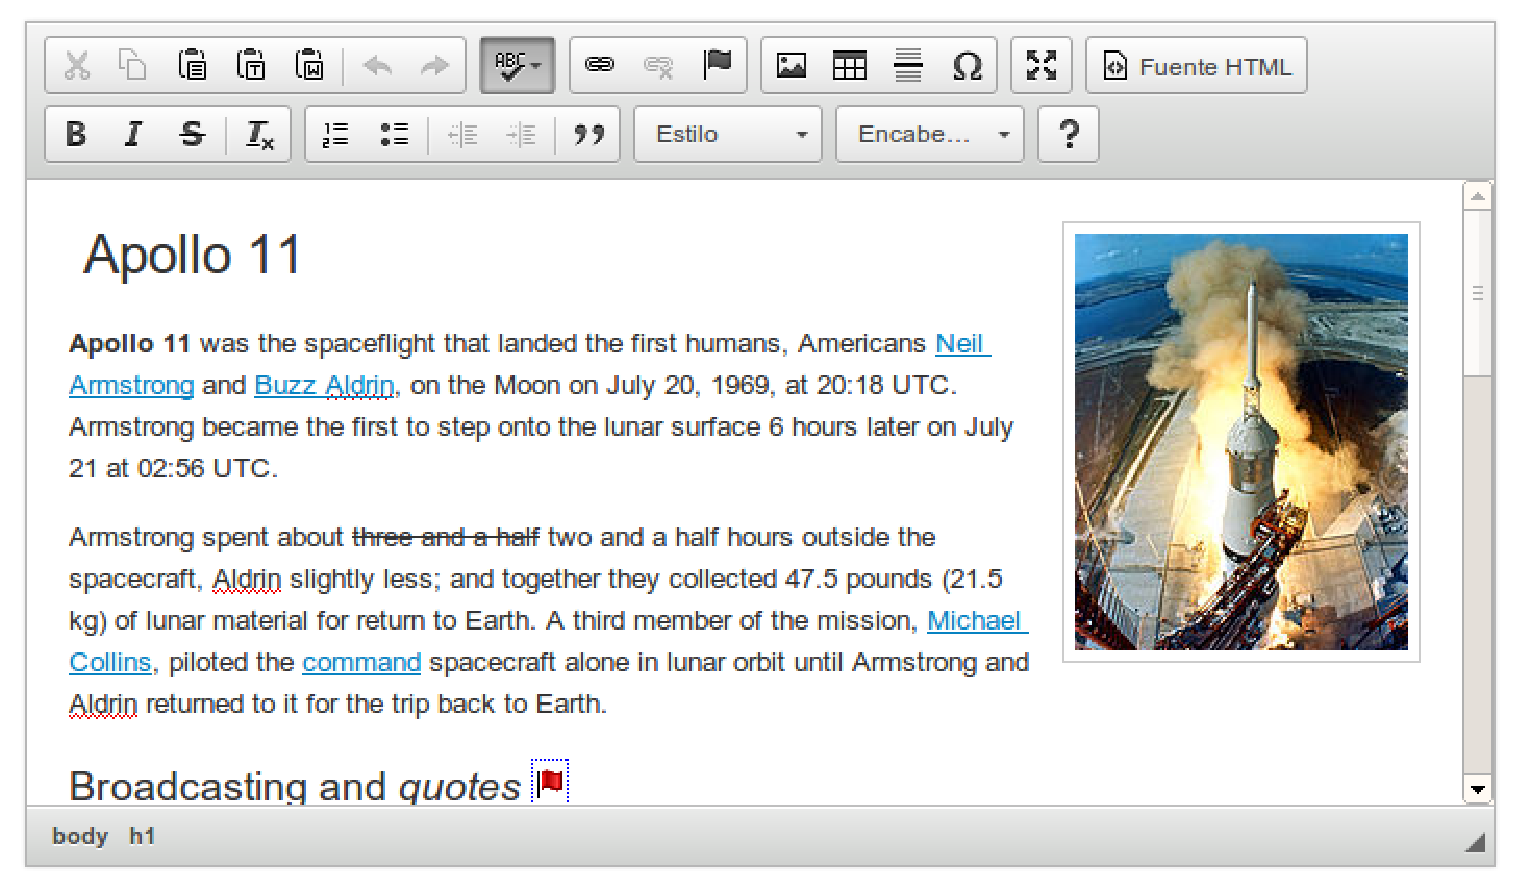
\includegraphics[width=1.0\textwidth]{fig/cke1}
  \caption{CKEditor}
\end{figure}

\subsection{openWYSIWYG}
\url{http://www.openwebware.com}
Este sencillo editor, distribuido bajo licencia de código abierto LGPL~\cite{LGPL:lgpl}, se presenta como el editor ideal para mejorar tu CMS. Como los anteriores remplaza textarea por un editor de texto. Parece ser que en la actualidad se encuentra obsoleto y presenta incompatibilidades con los navegadores actuales. Su web es \url{http://www.openwebware.com}.


\begin{figure}[h!]
  \centering
      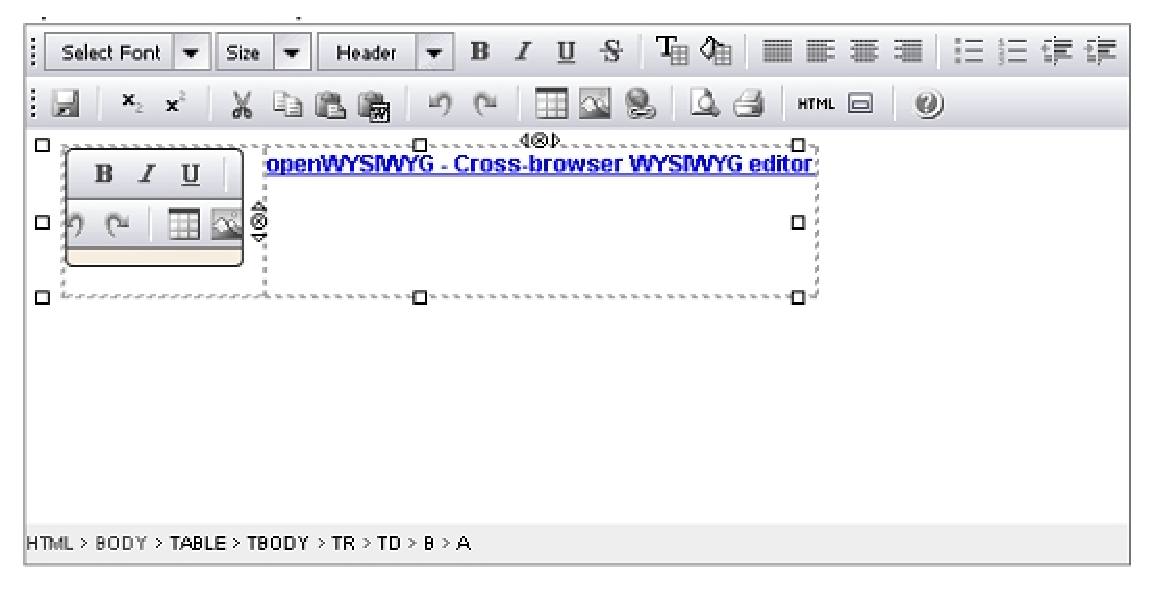
\includegraphics[width=1.0\textwidth]{fig/opene1}
  \caption{openWYSIWYG Editor}
\end{figure}


\section{Conclusiones del Análisis}

En este capítulo hemos analizado y reflexionado acerca de diversas plataformas y herramientas de la Web. A continuación veremos cuales de estas se ajustan más a nuestros objetivos, teniendo siempre en mente los requisitos de nuestro editor y buscando una solución sencilla y de calidad.

En lo referente a los editores descartamos el uso de \emph{openWYSIWYG} debido a los problemas de compatibilidad con los distintos navegadores que ha presentado, ya que parece ser que dicho editor se encuentra obsoleto.

Por otra parte hay algunos editores que soportan de forma nativa (o con el uso de plugins) el uso de fórmulas. Este es el caso de \emph{CKEditor} y \emph{YUI Rich Text Editor}.

\emph{CKEditor} es un proyecto maduro con 10 años en el mercado. Esta madurez se nota en todos los aspectos. El acabado de CKEditor es impecable, no tanto lo es el de sus plugins, desarrollados por terceros. A pesar de esto CKEditor es una opción muy a tener en cuenta. El problema que presenta, sin duda, es que esta complejidad de la que hace gala puede convertirse en un problema a la hora de estudiar y modificar su código fuente para adaptarlo a nuestras necesidades. Comentar también la posibilidad de usar cualquiera de las licencias ~\cite{GPL:gpl}, LGPL~\cite{LGPL:lgpl} y MPL~\cite{MPL:mpl}, lo que nos aporta gran libertad.
      
\emph{TinyMCE} supone una alternativa de calidad a \emph{CKEditor}. A diferencia de este último \emph{TinyMCE} se distribuye solo bajo licencia LGPL, lo que algunos casos podría ser una restricción. Sin embargo, en este caso concreto, no es importante ya que SWAD se encuentra liberado bajo una licencia AGPLv3 y no presentaría incompatibilidades con la licencia LGPL del editor. 

\emph{YUI Rich Text Editor} presenta una potente alternativa, con el respaldo de una gran empresa como es YAHOO. Como ya comentamos antes, se basa en el framework YUI (Yahoo User Interface), una serie de bibliotecas escritas en JavaScript para la construcción de aplicaciones de Internet enriquecidas (RIA) y liberadas bajo licencia BSD por parte de la compañía Yahoo. Sin embargo, para nuestro editor, evitaremos el uso de frameworks y nos basaremos en algún editor ``standalone''.

\emph{NicEdit} es una solución simple, aunque carece de soporte nativo para fórmulas, funcionalidad que tendríamos que ampliar con alguna otra herramienta, como puede ser MathJax o Texvc. A excepción de esto último, NicEdit implementa toda la funcionalidad necesaria por nuestro editor.

Al parecer, las mejores opciones para nuestro editor son NicEdit y CKEditor. CKEditor es mas pesado que NicEdit aunque mucho mas completo y con muchos plugins desarrollados por terceros. Dada la simplicidad del problema que nos ocupa, la ligereza de NicEdit es un gran punto a su favor, haciéndose innecesarios la gran mayoría de los plugins que tiene CKEditor. Por otra parte, el plugin WIRIS de fórmulas para CKEditor también está disponible para NicEdit. 

El problema de modificar un editor ya existente es que requiere una compleja labor de estudio de su código fuente para poder eliminar aquella funcionalidad que no necesitamos y añadir la funcionalidad de la que carece, así como adaptarlo a nuestros requisitos.  

Tras un completo análisis del código fuente de los editores se ha decidido implementar nosotros mismos el editor WYSIWYG, evitando el uso de cualquier Framework y desarrollando la solución lo más simple posible, cumpliendo cada uno de nuestros requisitos. Aunque no tomemos código fuente de ninguno de los editores anteriormente comentados, nos inspiraremos en NicEdit, el ligero editor que más se ajustaba a nuestras necesidades.




\chapter{Diseño del editor}

En este capítulo nos centraremos en los detalles concretos del diseño del editor. El editor resultante se compone de tres módulos bien diferenciados que son son el núcleo del editor, el editor de fórmulas y el purificador de HTML.

El núcleo del editor es un fichero Javascript que será el responsable de llevar a cabo la mayor parte de las funciones del editor. Este fichero encapsula la funcionalidad de la aplicación en la clase SwadeManager, SwadeDialog y SwadePanel. La primera de ella es una clase donde todos los métodos son estáticos y usamos para las distintas operaciones que componen la funcionalidad del editor. 

SwadeDialog es una clase que nos permite crear Dialog propios como el de la figura ~\ref{fig:dialog} y ofrece principalmente métodos para mostrarlos, ocultarlos y destruirlos.


\begin{figure}[h!]
  \centering
      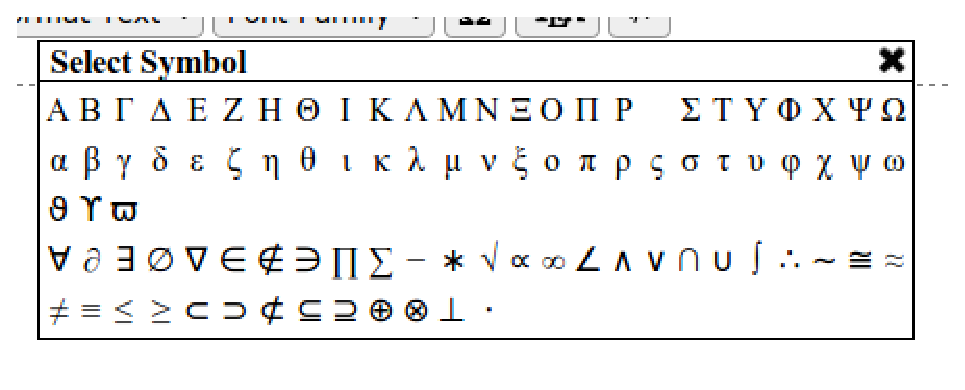
\includegraphics[width=4in]{fig/dialog}
  \caption{Dialogo creado con SwadeDialog.}
  \label{fig:dialog}

\end{figure}


SwadePanel es la clase que encapsula los métodos propios de cada editor. Estos métodos son principalmente para bloquear un editor cuando no se ha seleccionado y para el refresco del formato del texto seleccionado ~\ref{fig:panel}.

\begin{figure}[h!]
  \centering
      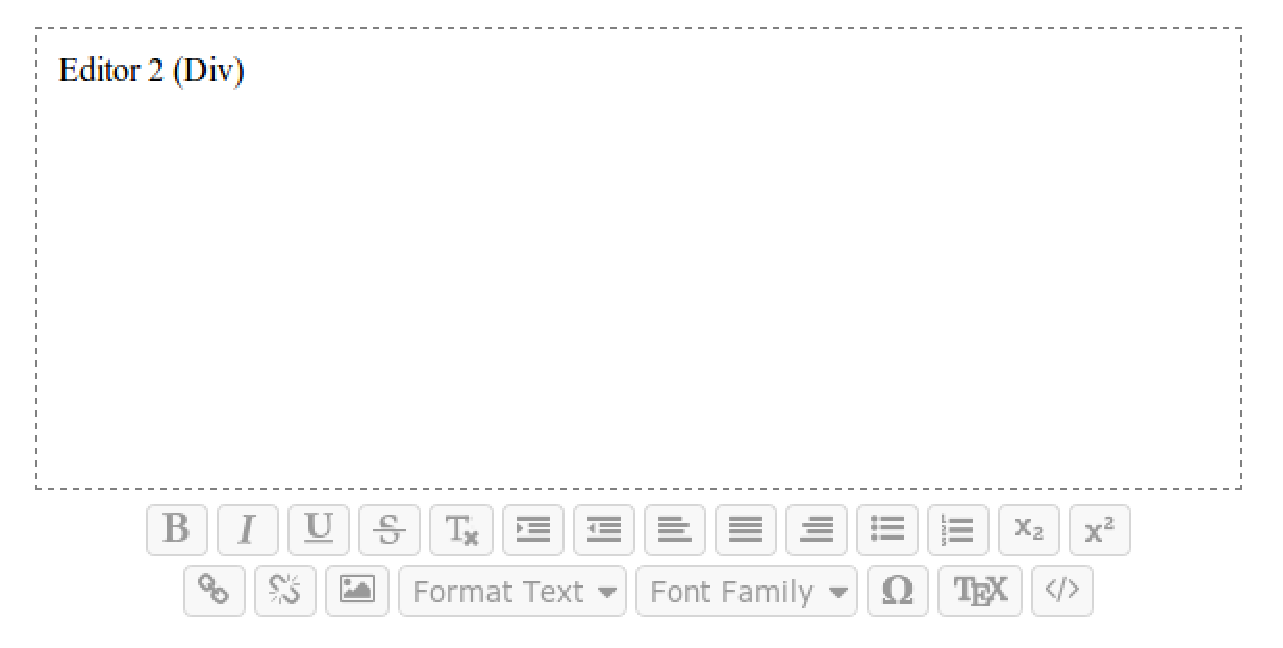
\includegraphics[width=7in]{fig/panel}
  \caption{Editor SWADE bloqueado.}
  \label{fig:panel}

\end{figure}


Para usar SWADE debemos incluir el fichero javascript con el código siguiente.

\begin{verbatim}
<script src="path-to-swade/swade.js" type="text/javascript"></script>
\end{verbatim}

Este script convierte uno o varios textarea o div en un editor SWADE. Para instanciar un editor en un textarea o div tenemos tres métodos. Por id, por clase o realizando una consulta. En el fragmento de código siguiente vemos un ejemplo de cada uno de ellos.

\begin{verbatim}
<script>
  SwadeManager.setOnDOMLoaded(function(){
  SwadeManager.setSwadeByQuery("textarea.swade"); //1
  SwadeManager.setSwadeById("swade-id");          //2
  SwadeManager.setSwadeByClassName("swade-class");//3
  }
  );
</script>
\end{verbatim}
La función SwadeManager.setOnDOMLoaded aplica la función pasada por parámetro cuando se ha construido completamente lo que se conoce por Document Object Model, aunque las imágenes aún estén en carga.
A esta función le pasaremos los métodos para instanciar el editor en las distintas partes de la página. Con el primero de ellos instanciaremos un editor en aquellos textarea con la clase ``swade'', con el segundo lo haremos para los elementos div o textarea con id ``swade-id'' y con el último instanciaremos el editor para los elementos div o textarea con clase ``swade-class''. 

Todas estas funciones se apoyan en las distintas funciones de selección de Javascript y la función setSwade, que instancia un editor para cada elemento de un vector de elementos. En esta función se tiene en cuenta si el objetivo es un div o un textarea, siendo este último el caso más complejo. Si el objetivo es un div se añade a este un panel al que añadimos los distintos eventos de pulsación de los distintos botones. Por el contrario, si el objetivo es un textarea, debemos crear nosotros mismo el elemento div, asignarle como contenido el valor del textarea, ocultar dicho textarea y comprobar si formaba parte de un formulario. Si el textarea formaba parte de un formulario, debemos interceptar la petición del formulario para establecer el valor del textarea al valor del div que estamos editando. 


El editor de fórmulas es una página HTML que usa la herramienta Mathjax para renderizar la fórmula en tiempo real usando HTML y CSS. Este proceso se lleva a cabo mientras que el usuario la escribe dicha fórmula. 

Cuando el usuario finaliza la inserción de la fórmula, enviamos una petición asíncrona al servidor al script tex2png.php que nos devolverá el elemento HTML correspondiente a la imagen generada. El fragmento de código siguiente es el responsable de hacer la petición al servidor de forma asíncrona, de insertar la imagen devuelta por este en SWADE y de cerrar la ventana del editor de fórmulas. 

\begin{verbatim}

function showFormula(str)
{
    var xmlhttp;
    if (window.XMLHttpRequest)
    {// code for IE7+, Firefox, Chrome, Opera, Safari
        xmlhttp=new XMLHttpRequest();
    }
    else
    {// code for IE6, IE5
        xmlhttp=new ActiveXObject("Microsoft.XMLHTTP");
    }
    xmlhttp.onreadystatechange=function()
    {
        if (xmlhttp.readyState==4 && xmlhttp.status==200)
        {
            opener.tex = xmlhttp.responseText;
            window.returnValue = xmlhttp.responseText;
            top.close();
            return false;
        }
    }
    xmlhttp.open("POST","tex2png.php",true);
    xmlhttp.setRequestHeader("Content-type","application/x-www-form-urlencoded");
    xmlhttp.send("MathInput="+encodeURIComponent(str));

}

\end{verbatim}

Para el editor de fórmulas, en la parte del servidor, encontramos el script tex2png.php (que no tiene nada que ver con la herramienta tex2png descrita en el capítulo \emph{Estado del arte}).

Este script se ocupa de extraer el valor de la fórmula de la variable POST, de generar la imagen correspondiente con texvc y de devolver el elemento HTML necesario para insertar dicha fórmula en nuestro editor SWADE. El fragmento de código siguiente recoge dicha funcionalidad.

\begin{verbatim}
...
$latex_formula = "'".$_POST["MathInput"]."'";
$cadena = "./texvc $path_tmp $path_dest $latex_formula";
exec($cadena,$output,$return);
...
echo "<img src=\"${cwd}/${path_dest}${name}.png\" alt=\"Formula inválida\" 
data-tex-swade = $latex_formula 
onclick=\"swade_app.tex_code_selected = $latex_formula;\
swade_app.selected_tex_object = this;\" 
style=\"vertical-align:middle;\"/>";
\end{verbatim}

Podemos observar como se han añadido algunos atributos al elemento HTML para insertar la imagen, aparte de la ruta de esta. El atributo data-tex-swade y onclick son para poder editar la fórmula haciendo click sobre ella. El atributo style es para alinear la fórmula con el texto que la rodea.


El último modulo de nuestro editor es la herramienta HTMLpurifier~\cite{htmlpurifier}, la cual se ocupará del filtrado del HTML generado por el usuario. Dicha herramienta está escrita en php y nos permitirá evitar ataques XSS en la página de la plataforma. En el siguiente fragmento de código se muestra un ejemplo de uso de dicha herramienta.

\begin{verbatim}
...
require_once '../htmlpurifier/library/HTMLPurifier.auto.php';
$config = HTMLPurifier_Config::createDefault();
$config->set('Core.Encoding', 'UTF-8'); 
$config->set('HTML.Doctype', 'HTML 4.01 Transitional'); 
$purifier = new HTMLPurifier($config);
...
$parsed_content = $purifier->purify($_POST['editor3']);
...
\end{verbatim}

Para usar dicha herramienta debemos instanciar el purificador con una configuración determinada y finalmente aplicar el método purify sobre el texto que queremos purificar. Dado que la plataforma usa la codificación ISO-8859-1, en este punto tendremos que tener en mente una serie de consideraciones recogidas en el apéndice \emph{Integración en la plataforma SWAD}.


%\chapter{Integración en SWAD}

Modulos:
- Editor JS
- Sustitutitución de divs por Swade
- Limpieza de html producido en el Servidor
Ejemplo:
static string SanitizeHtml(string html)
{
    string acceptable = ``script|link|title'';
    string stringPattern = @''</?(?(?='' + acceptable + @'')notag|[a-zA-Z0-9]+)(?:\s[a-zA-Z0-9\-]+=?(?:([",']?).*?\1?)?)*\s*/?>'';
    return Regex.Replace(html, stringPattern, ``sausage'');
}

%\chapter{Pruebas realizadas}

En este capítulo se detallan las pruebas realizadas sobre las distintas herramientas y editores, así como su instalación y la integración de varias de ellas formando una única solución.

El objetivo de estas pruebas no es otro que el de obtener la solución idónea y no tener que arrepentirnos más tarde de la opción escogida, con la pérdida de tiempo que eso conllevaría. Además, de esta forma nuestro editor será una solución mucho más madura debido a este tiempo que emplearemos en reflexionar sobre lo que hemos llamado state-of-the-art.

Cómo ya dijimos previamente, no se trata de reinventar la rueda. Muchos de los editores analizados dan soluciones muy buenas al problema del editor WYSIWYG, además de ser proyectos estables con algunos años en desarrollo. 

Lo mejor de todo es que la mayoría de las herramientas analizadas se distribuyen bajo licencias de software libre, lo que nos da libertad de ejecutar, copiar, distribuir, y estudiar el mismo, e incluso modificar el software y distribuirlo modificado. 

\section{Prueba de editores}
\subsection{CKEditor}
\section{Prueba MathJax}
\section{Pruebas Soporte Fórmulas}
\subsection{Generador de fórmulas AJAX con tex2png}
Se implementó un generador de fórmulas en el que mientras el usuario escribe el código {\LaTeX} se generan peticiones al servidor que va enviando al cliente imágenes, renderizando el código escrito. 

El problema de esta solución es el gran número de imágenes (temporales) generadas en el servidor las cuales posteriormente deberían de ser eliminadas.

Otro problema acontecido fué la generación errónea de imágenes por parte de tex2png, por ellos nos planteamos usar la herramienta texvc.

\subsection{Generador de fórmulas usando MathJax y texvc}

\section{Pruebas de integración}
\subsection{NicEdit + MathJax}

Como primera aproximación de nuestro editor WYSIWYG se pensó en la unificación del editor NicEdit junto con MathJax. Dicho editor fué bautizado como Nax y como punto fuerte cuenta con su sencillez de uso y de integración.

La primera prueba realizada fue una página en la que introducimos texto en un editor NicEdit, pudiendo incluir también formulas en {\LaTeX} y al hacer submit del formulario se muestra en la página el texto introducido y las formulas renderizadas, si es que habiamos escrito alguna.

\begin{figure}[h!]
  \centering
      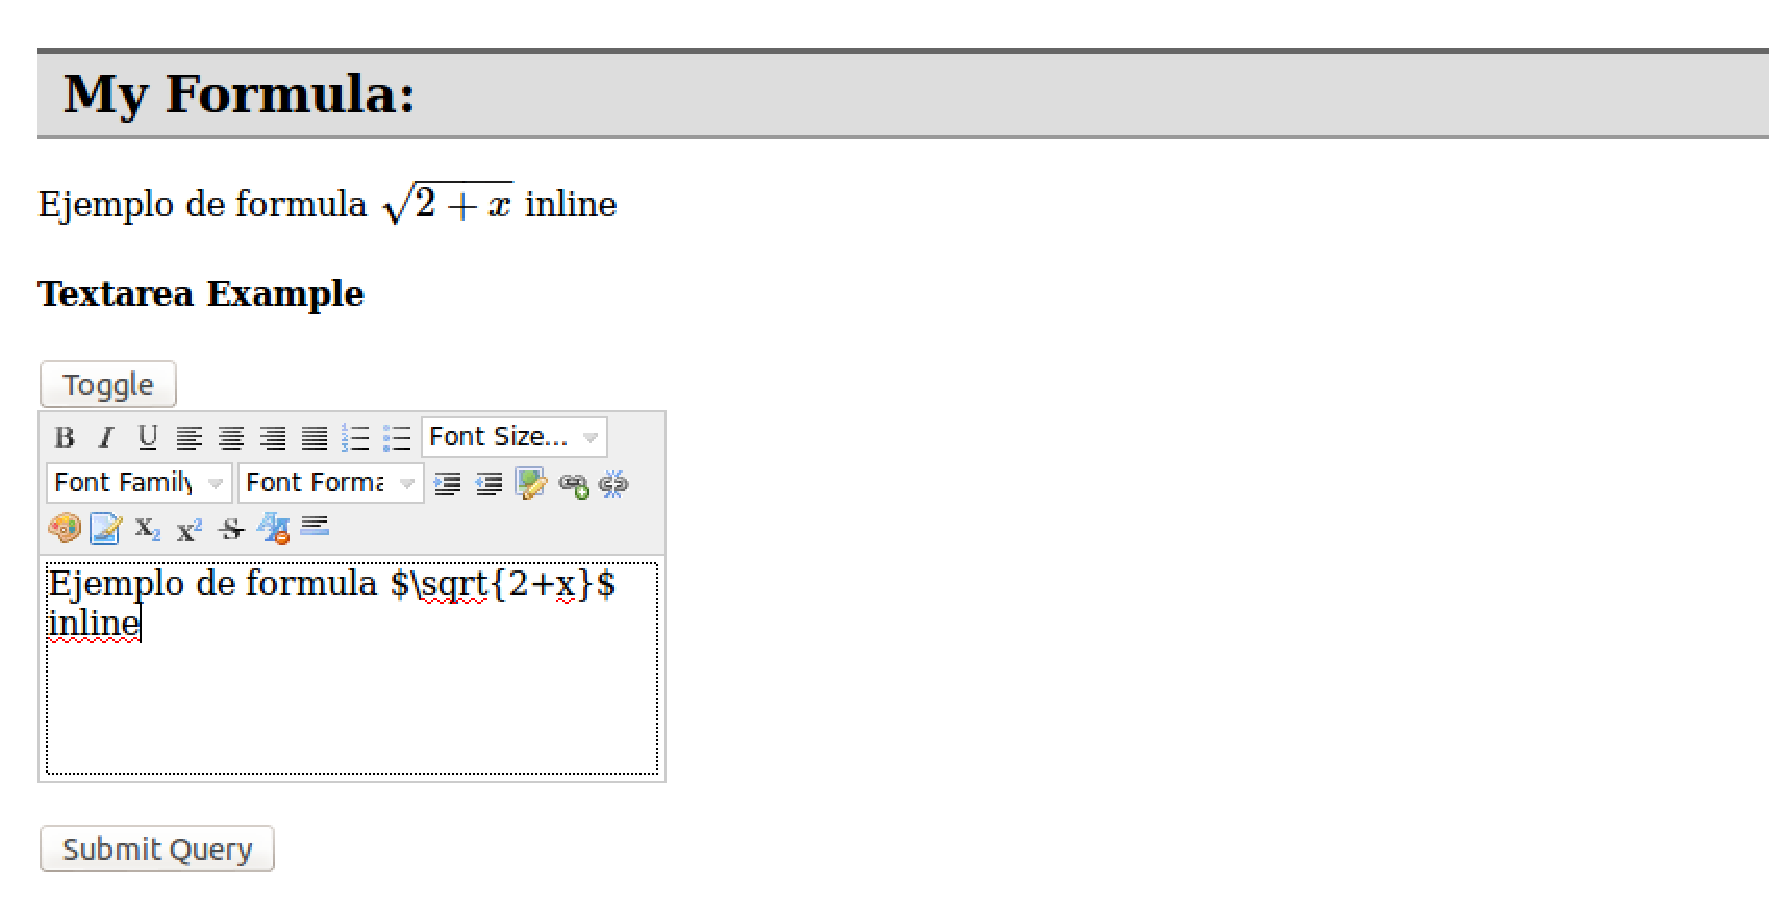
\includegraphics[width=0.9\textwidth]{fig/nax1}
  \caption{Prueba 1 : Nax Editor}
\end{figure}

Cabe destacar de esta primera propuesta su sencillez y calidad final demostrándose la facilidad con la que se integran ambas herramientas.

\subsection{NicEdit + WIRIS Plugin}

\chapter{Resultados}

El editor resultante es un editor ligero y fácil de usar que puede insertarse en una página con apenas dos líneas de código (ver apéndice Integración en la plataforma SWAD). Se han realizado una serie de pruebas sobre el editor y aunque aún no se ha incorporado totalmente en la plataforma se han obtenido muy buenos resultados.

Durante el desarrollo del editor se han ido realizando pruebas en la página de test de la figura ~\ref{fig:result_testpage0}.

\begin{figure}[h!]
  \centering
      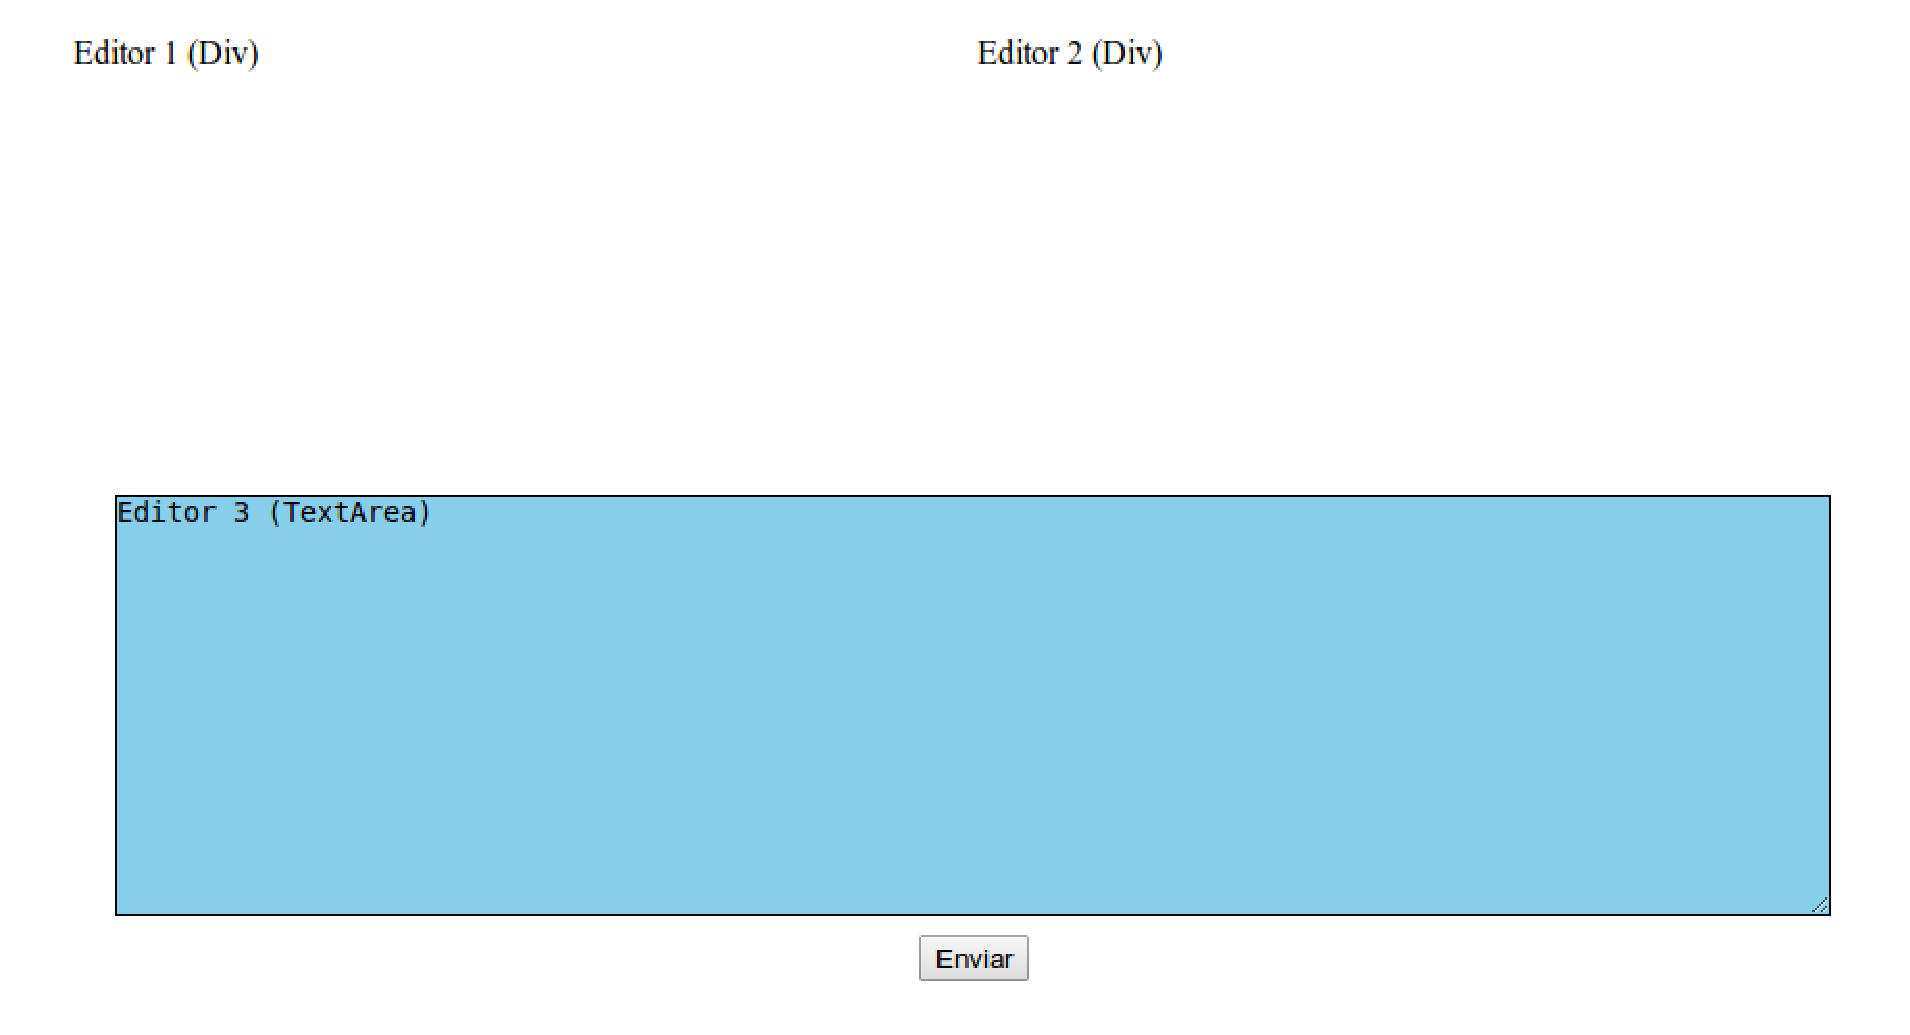
\includegraphics[width=7in]{fig/result_testpage0}
  \caption{Página de pruebas sin SWADE}
  \label{fig:result_testpage0}

\end{figure}


Esta página posee dos elementos div y un textarea, identificados por el atributo HTML clase ``swade''. Insertando en la cabecera de la página las líneas de código siguientes:
\begin{verbatim}
<script src="../swade.js" type="text/javascript"></script>
<script>
  SwadeManager.setOnDOMLoaded(function(){
  SwadeManager.setSwadeByClassName("swade");});
</script>
\end{verbatim}

Nuestro editor hará el resto del trabajo, transformando los tres elementos citados en editores SWADE. Ver figura ~\ref{fig:result_testpage1}.

\begin{figure}[h!]
  \centering
      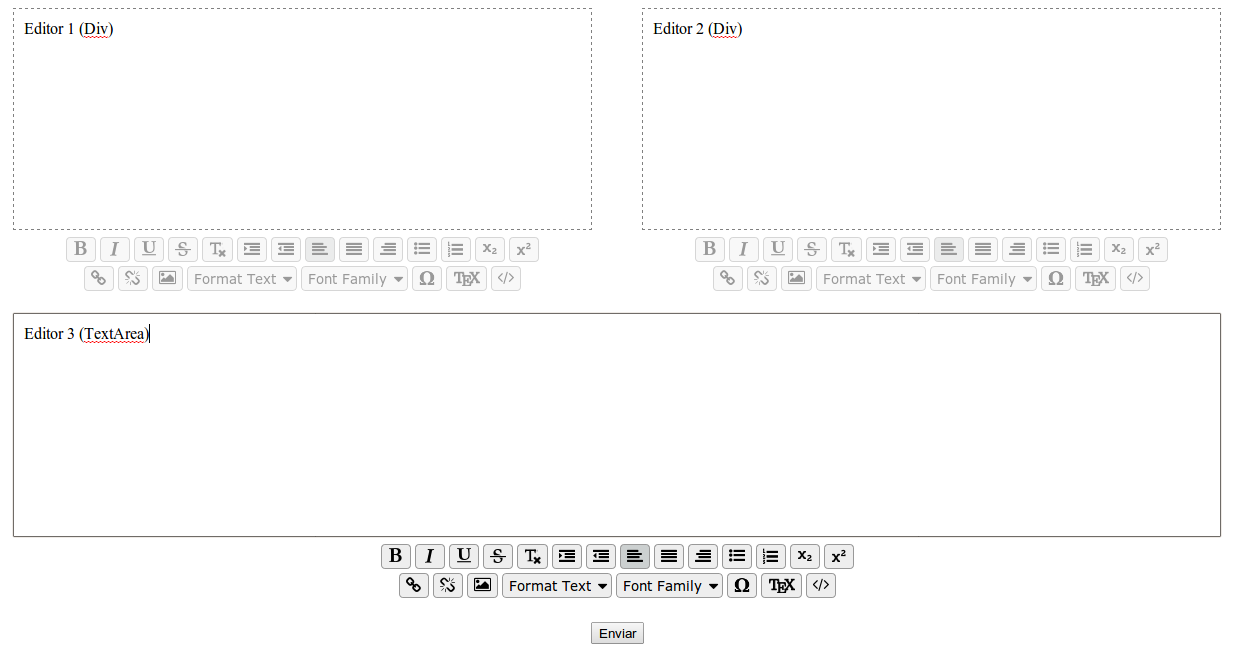
\includegraphics[width=7in]{fig/result_testpage1}
  \caption{Página de pruebas con SWADE}
  \label{fig:result_testpage1}

\end{figure}


Esta página contiene también un formulario cuyos únicos elementos son el textarea inferior y el botón de submit, responsable de enviar el contenido del textarea. Nuestro editor se ocupará de interceptar el evento de pulsación del botón para asignar el contenido del editor al textarea antes de ser enviado. De esta forma se enviará el código HTML que contiene el editor.

\begin{figure}[h!]
  \centering
      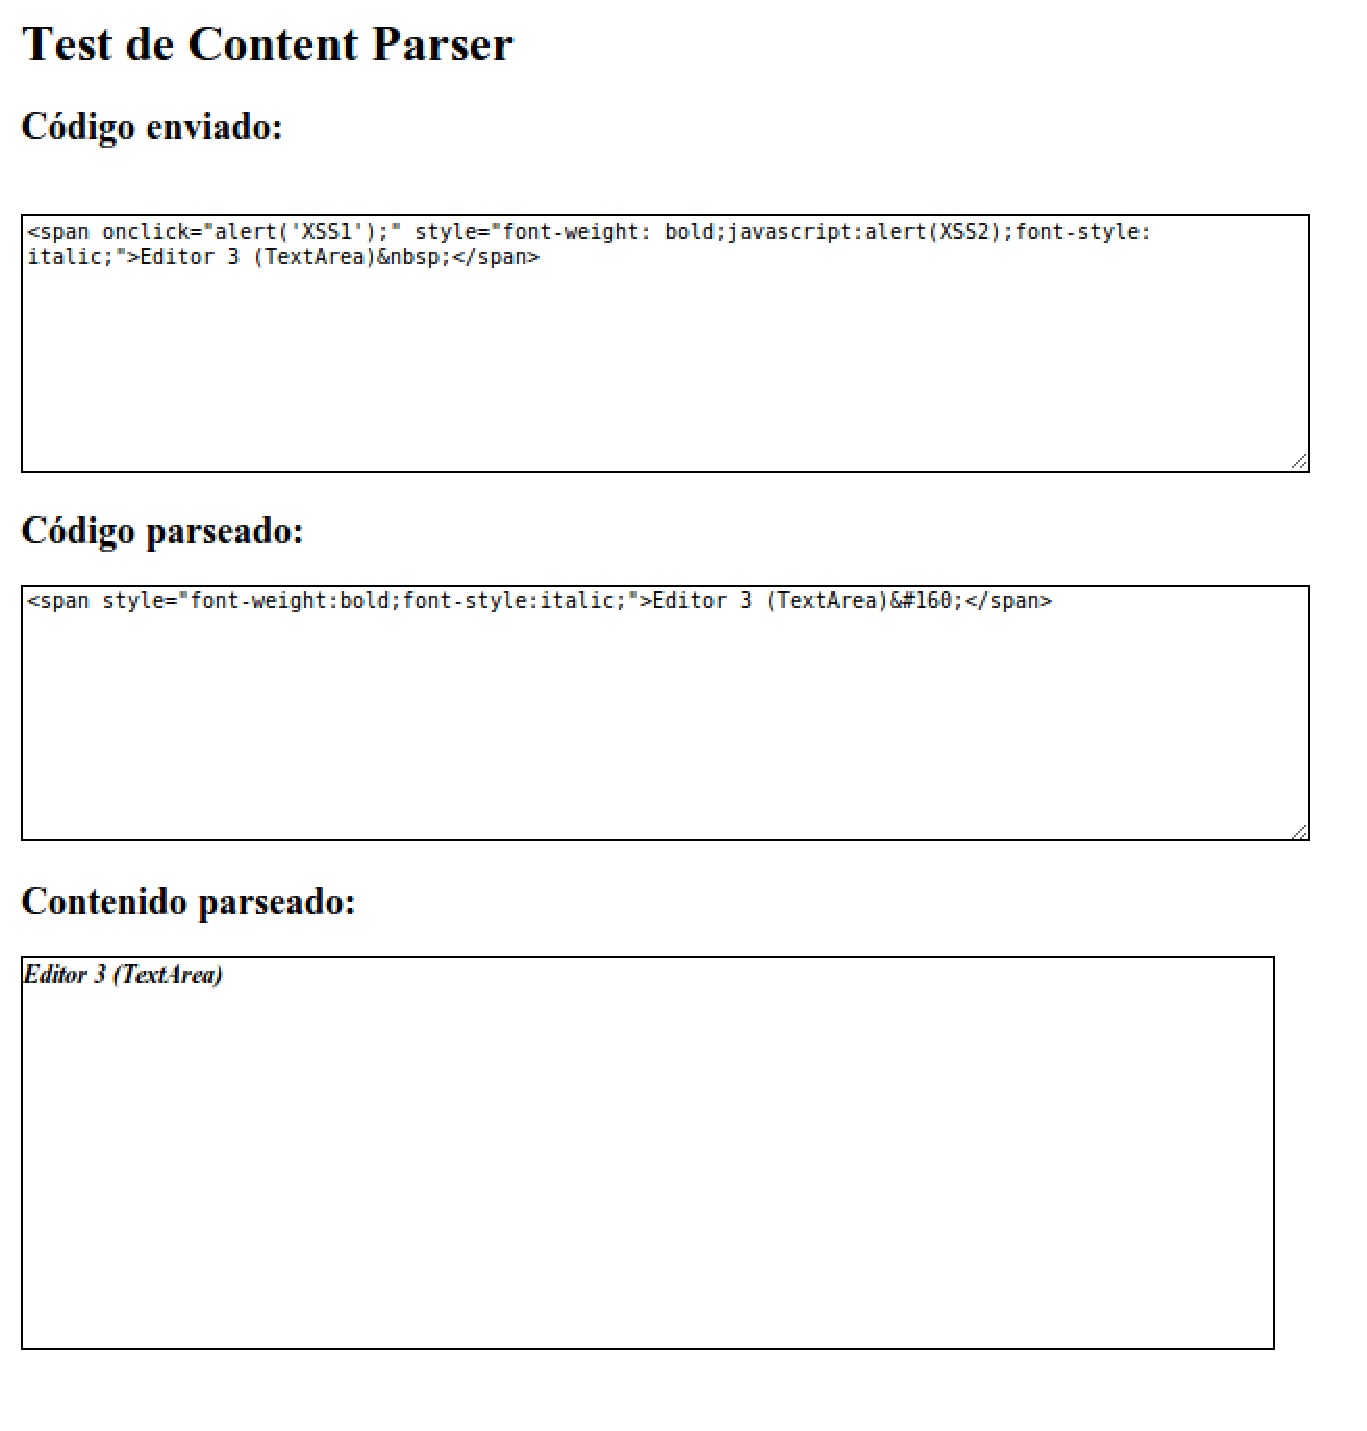
\includegraphics[width=5in]{fig/result_testpage2}
  \caption{Páginas de pruebas de limpieza HTML}
  \label{fig:result_testpage2}
\end{figure}

Para probar el filtrado HTML se ha usado la página de las figura ~\ref{fig:result_testpage2}. Esta página es un script php que recoge el valor enviado por el formulario y muestra su valor filtrado y sin filtrar, además de renderizar el HTML filtrado.


En las figuras ~\ref{fig:result_testpage3} y ~\ref{fig:result_testpage4} podemos ver el envío de símbolos y fórmulas.

\begin{figure}[h!]
  \centering
      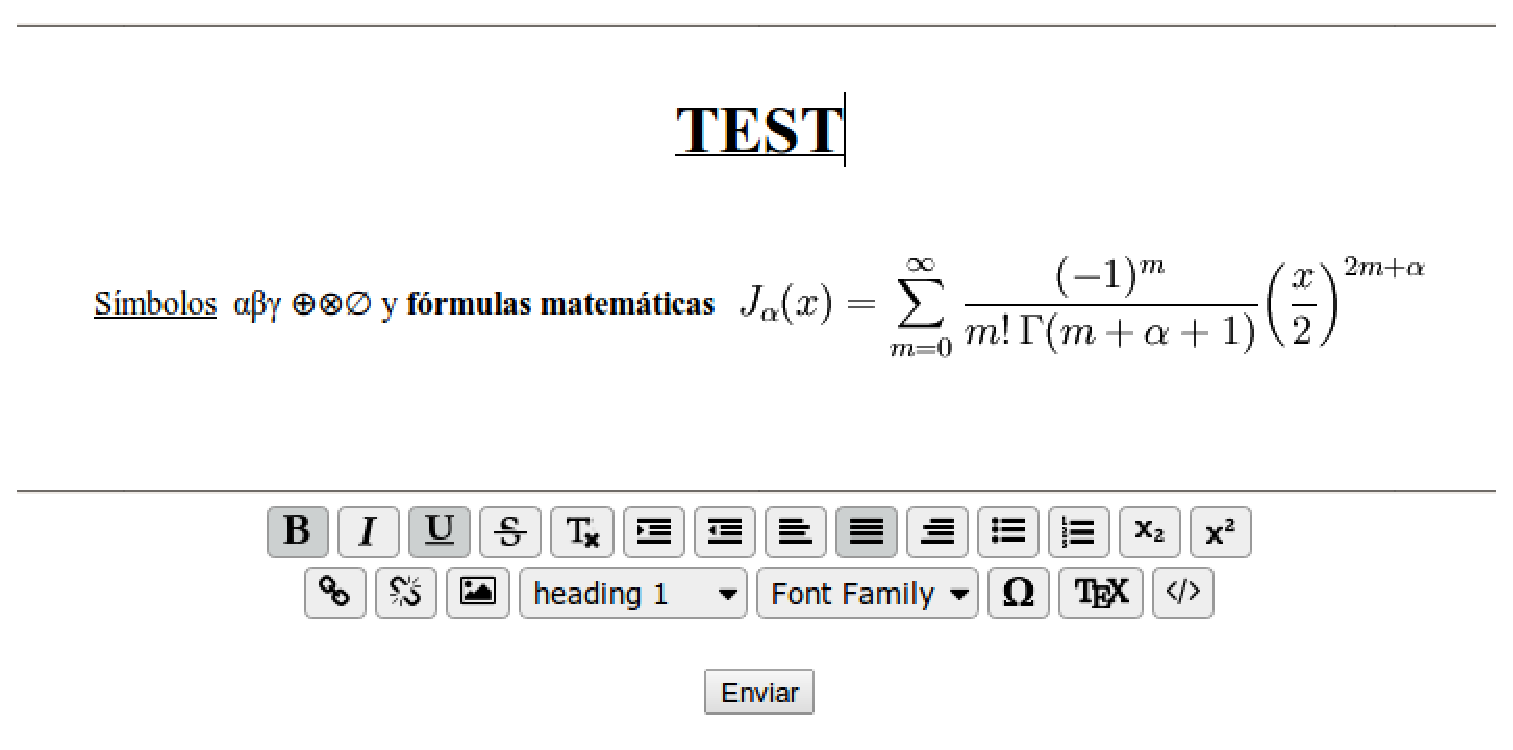
\includegraphics[width=5in]{fig/result_testpage3}
  \caption{Envío en un formulario de símbolos y fórmulas.}
  \label{fig:result_testpage3}

\end{figure}


\begin{figure}[h!]
  \centering
      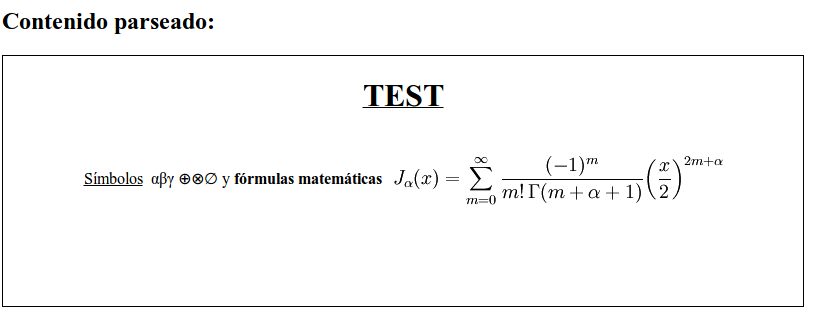
\includegraphics[width=5in]{fig/result_testpage4}
  \caption{Limpieza del HTML en el servidor y renderizado del contenido enviado en el formulario.}
  \label{fig:result_testpage4}

\end{figure}

Una vez testeada la funcionalidad del editor, hicimos algunas pruebas de integración en las secciones descritas en el capítulo de Análisis. 

En la figura ~\ref{fig:swade_test1} podemos ver el editor integrado en la sección de envío de mensajes y en las figuras ~\ref{fig:result_test1} y ~\ref{fig:result_test2} lo vemos en la sección de Test. 

\begin{figure}[h!]
  \centering
      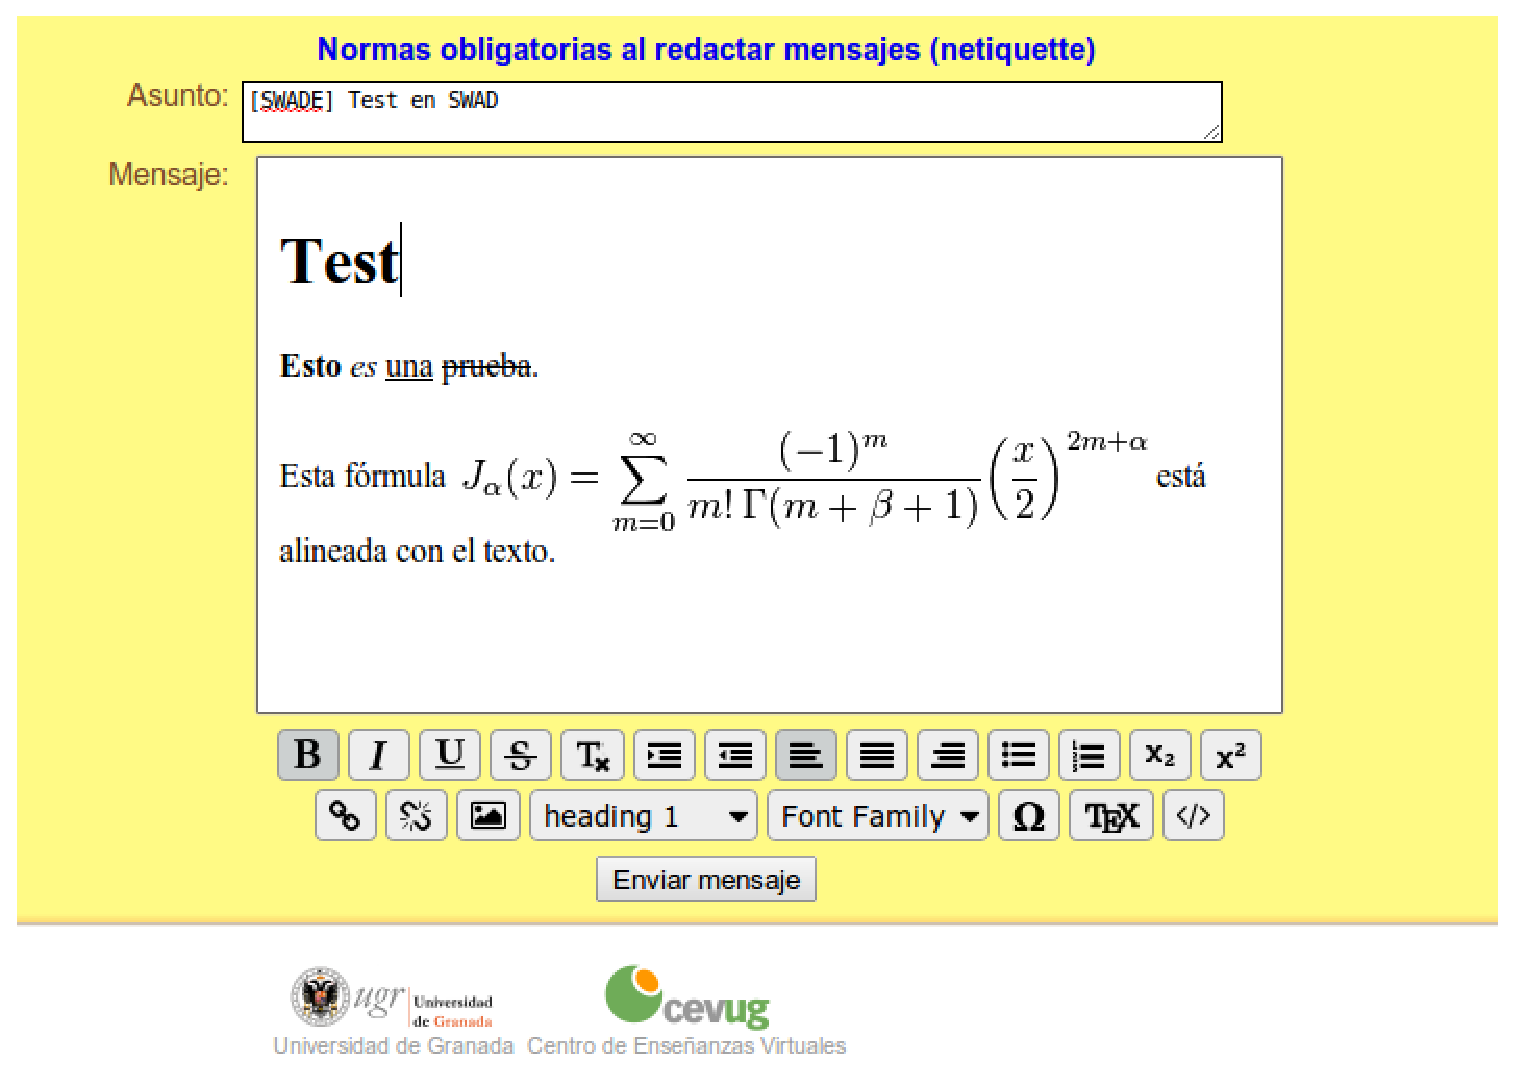
\includegraphics[width=5in]{fig/swade_test1}
  \caption{SWADE en mensajes}
  \label{fig:swade_test1}

\end{figure}


\begin{figure}[h!]
  \centering
      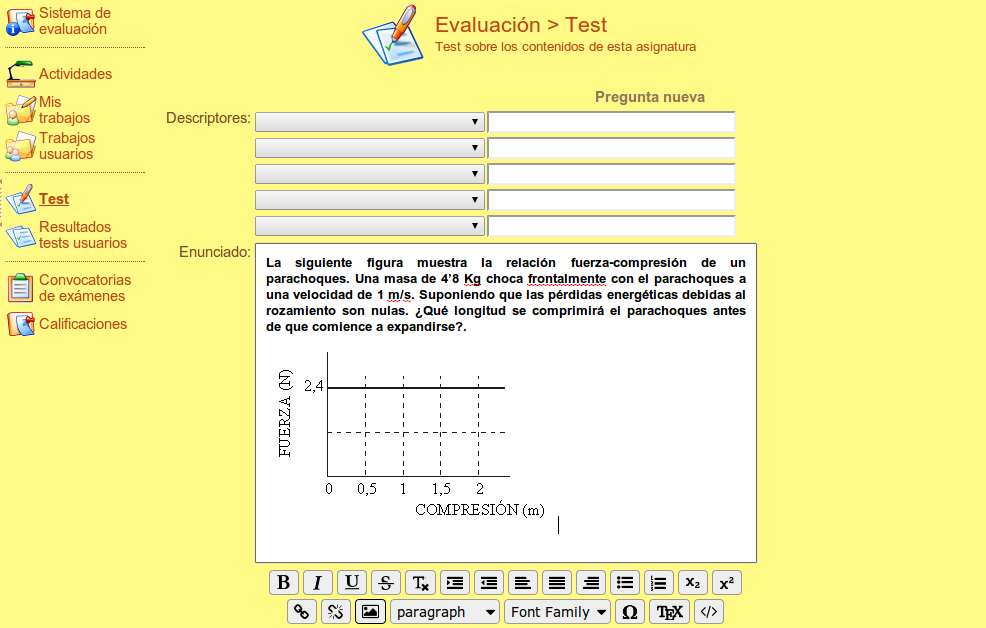
\includegraphics[width=5in]{fig/result_test1}
  \caption{SWADE en preguntas de Test}
  \label{fig:result_test1}

\end{figure}


\begin{figure}[h!]
  \centering
      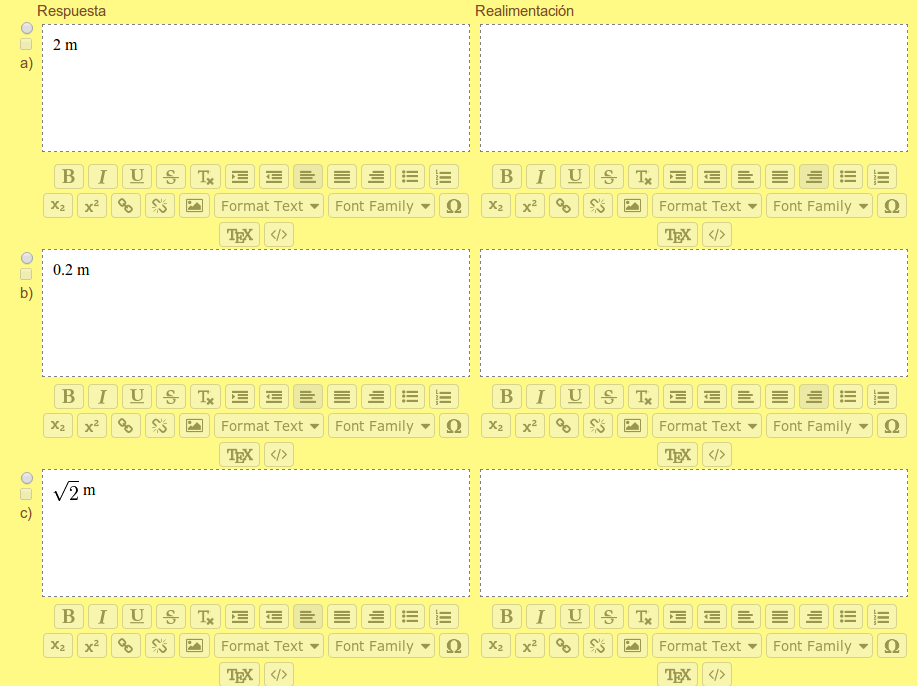
\includegraphics[width=5in]{fig/result_test2}
  \caption{SWADE en respuestas de Test}
  \label{fig:result_test2}

\end{figure}



\chapter{Conclusiones}

Existe un mundo de posibilidades en el mercado laboral en lo que a aplicaciones web se refiere. Aunque con los conocimientos adquiridos en la carrera se puede aprender una tecnología concreta en un tiempo razonable, si bien es verdad que al inicio de tu vida laboral te piden experiencia en ciertas herramientas que en muchos casos no has adquirido.

Por eso, una de mis motivaciones para la elección de este proyecto de fin de carrera era aprender todo lo posible acerca de aplicaciones web y las tecnologías actuales para su desarrollo. En este punto me siento muy satisfecho con el trabajo desarrollado, ya que a lo largo del año he adquirido conocimientos de tecnologías concretas como son HTML, PHP y Javascript y metodologías de desarrollo como AJAX entre otras. Además del aprendizaje y la experiencia de tecnologías específicas, también he aprendido mucho acerca de aplicaciones web, lo que facilitará mi aprendizaje futuro de otras herramientas. 

En una fase inicial me dediqué al aprendizaje de las distintas herramientas para el desarrollo del editor. He aprendido mucho de la web \url{http://w3schools.com/} y debo mucho a la comunidad de desarrolladores de \url{http://stackoverflow.com/}, conocimiento que espero poder devolver en algún momento.

Mi segunda motivación era la resolución de un problema real, construir algo que sirviera a la gente, y que no se quedara en el CDROM de la estantería de un departamento de la ETSIIT. Por este motivo me puse en contacto con Antonio Cañas, pues soy consciente de la amplia difusión de SWAD en la UGR, y me ofrecí para llevar a cabo alguna de las ideas que tuviera en mente para mejorar dicha plataforma.

Es distinto el desarrollo de software para unas prácticas de una asignatura que desarrollarlo para su uso en una plataforma real, que será usada al día por cientos de personas. Lo que en unas prácticas es secundario (para subir nota), aquí es primordial y la atención a los pequeños detalles lo es todo. He pasado muchas horas solucionando pequeños errores sutiles o trabajando para que el editor funcione sin problemas en los distintos navegadores más usados. También he pasado muchas horas leyendo foros y FAQs y trabajando en la configuración de las herramientas externas como texvc y HTMLpurifier para conseguir que funcionaran correctamente. Los detalles de dicha configuración pueden encontrarse en los apéndices.  

Puede probarse la versión final del editor en una página de test en \url{http://openswad.org/swade/test/}. La solución que propongo aún necesita pasar algunas pruebas antes de estar completamente integrada en la plataforma, pero continuaré colaborando junto con Antonio Cañas para su completa implantación. Es por este motivo por el que he liberado el código fuente de SWADE con la licencia Affero GPL y se puede descargar de \url{https://github.com/asce/swade}, de forma que cualquiera que esté interesado podrá colaborar en la mejora del editor.


%============================================================
%   Apéndices
%============================================================
\renewcommand{\appendixtocname}{APÉNDICES}%Cambia el nombre de toc para apéndices
\renewcommand{\appendixpagename}{APÉNDICES}%Cambia el nombre para la página
\renewcommand{\appendixname}{APÉNDICE}
\appendix
\addappheadtotoc
\appendixpage
%\include{codigo}
\chapter{Instalación en el Servidor de OpenSWAD}

El servidor donde se encuentra OpenSWAD usa una instalación mínima del SO Linux CentOS 5.7 en su versión de 64 bits. SWADE usa distintas herramientas libres para desarrollar parte de su funcionalidad. Estas herramientas son HTMLpurifier~\cite{htmlpurifier}, texvc~\cite{texvc} y MathJax~\cite{mathjax}, ya comentadas anteriormente. A continuación describiremos el proceso de instalación de dichas herramientas.

En primer lugar instalamos mediawiki y la última versión de php en el servidor. Mediawiki se usará para una futura implementación de una wiki para OpenSWAD, lo cuál no pertenece al ámbito de este documento. La instalación de php, sin embargo, era necesaria ya que actualmente no se usa php en la plataforma y nos será de utilidad para algunas de las funciones que vamos a desarrollar.

HTMLpurifier se usa para filtrar el código HTML generado y protegernos de la inyección de posible código malicioso. Deberá instalarse en el fichero raíz de SWADE como htmlpurifier. La página de dicha herramienta es: http://htmlpurifier.org/. Será necesario configurar la codificación de caracteres y doctype en el fichero content\_parser.php. Existe un ejemplo de uso de la función de filtrado en test/form.php.

Para usar la caché de HTMLpurifier será necesario dar permisos de escritura a los directorios que cuelgan de library/HTMLPurifier/DefinitionCache/Serializer. Para ello usaremos el comando: 

\begin{verbatim}
chmod -R 0755 library/HTMLPurifier/DefinitionCache/Serializer
\end{verbatim}

Texvc se usa para generar las imágenes de las formulas LaTeX y forma parte de la extensión math de mediawiki. Antes de compilar dicha herramienta debemos instalar sus dependencias, que son:
\begin{itemize}
\item ocaml
\item LaTeX
\item dvipng
\end{itemize}

La última ya se encuentra instalada así que nos centramos en la instalación de las otras dos. 

Para instalar ocaml descargamos las fuentes de su página oficial (\url={http://caml.inria.fr/download.en.html}) y a continuación la compilamos e instalamos con los siguientes comandos:

\begin{verbatim}
./configure
make world
make opt
sudo make install
make clean
\end{verbatim}

LaTeX podemos instalando usando el gestor de paquetes yum mediante el comando: \begin{verbatim}yum install tetex\end{verbatim}

Finalmente para la compilación de la herramienta texvc, una vez resueltas sus dependencias, nos bajamos la extensión math de mediawiki de su página: \url{http://www.mediawiki.org/wiki/Special:ExtensionDistributor?extdist_extension=Math}. 
Una vez descargados los ficheros fuente, accedemos al directorio math/ y ejecutamos el comando: \begin{verbatim}make\end{verbatim}

Será necesario copiar el binario generado dentro del directorio tex\_editor, que se encuentra en el directorio raíz de SWADE.


Deberemos compilar dicha herramienta e incluirla en la carpeta tex\_editor (o en el path). Para la generación de las imágenes de las fórmulas debemos dar permisos de escritura a las carpetas tex\_editor/img y tex\_editor/tmp. Podemos modificar la localización de estas carpetas en el script php tex\_editor/tex2png.php. Para más información acerca de texvc consultar: \url{http://www.mediawiki.org/wiki/Texvc} 

En el caso de no generarse correctamente las imágenes de las fórmulas debemos consultar si tenemos instalados las herramientas latex, dvips, gs y convert (ImageMagick).

\begin{verbatim}
which latex
which dvips
which gs
which convert
\end{verbatim}

En nuestro caso tuvimos que instalar ImageMagick con:

\begin{verbatim}
yum install ImageMagick
\end{verbatim}

Si se generan los archivos temporales .tex pero no se genera la imagen el problema puede solucionarse copiando a la carpeta de los archivos temporales el fichero latex.fmt. Este fichero puede estar en varios sitios, en nuestro caso se encontraba en ~/.texmf-var/web2c/latex.fmt. En caso de no aparecer en dicha ruta usar el comando find.

\begin{verbatim}
find ~ -name latex.fmt
\end{verbatim}

Para cualquier otro problema en el uso de texvc consultar \url{http://www.mediawiki.org/wiki/Manual:Enable_TeX/problems}.

 
Para la visualización de las fórmulas LaTeX mientras el usuario escribe su código se usa la herramienta MathJax. Dicha herramienta deberá instalarse en la carpeta tex\_editor de SWADE. La página de dicha herramienta es http://www.mathjax.org/


\chapter{Integración en la plataforma SWAD}
Insertar SWADE en una página web es tan sencillo como incluir el fichero swade.js en la página y elegir uno de los tres métodos que ofrece para instanciar este en los textarea o div.

\begin{verbatim}
<script src="path-to-swade/swade.js" type="text/javascript"></script>
<script>
SwadeManager.setOnDOMLoaded(function(){
  SwadeManager.setSwadeByQuery("textarea.swade"); //1
  SwadeManager.setSwadeById("swade-id");          //2
  SwadeManager.setSwadeByClassName("swade-class");//3
}                      
);
</script>  
\end{verbatim}

Con el primero de ellos instanciaremos un editor en aquellos textarea con la clase ``swade'', con el segundo lo haremos para los elementos div o textarea con id ``swade-id'' y con el último instanciaremos el editor para los elementos div o textarea con clase ``swade-class''.

Sin embargo, a la hora de integrar SWADE en la plataforma SWAD uno de los mayores problemas al que nos enfrentamos es la codificación de caracteres. Nuestro editor permite la introducción de caracteres Unicode (UTF-8) mientras que SWAD usa una codificación ISO Latin 1 (iso-8859-1) por lo que tendremos que tener especial cuidado en el tratamiento del código HTML generado por el usuario.

Si queramos enviar el contenido de un editor usando un formulario deberemos asignarle al atributo accept-charset el valor ``iso-8859-1''. De esta forma nos aseguramos que envíe como entidad los caracteres Unicode que ISO Latin 1 no reconoce. 

\begin{verbatim}
<form action="form.php" accept-charset="iso-8859-1">
...
</form>
\end{verbatim}

De la misma manera, en el servidor, tendremos que codificar los caracteres desconocidos con entidades cuando accedamos al valor que hemos enviado en el formulario. Pero antes de realizar esta tarea debemos asegurarnos de sanear el HTML para evitar ataques XSS~\cite{xss}.

Para realizar esta tarea debemos crear el purificador:

\begin{verbatim}
require_once '../htmlpurifier/library/HTMLPurifier.auto.php';
$config = HTMLPurifier_Config::createDefault();
$config->set('Core.Encoding', 'ISO-8859-1'); // replace with your encoding
$config->set('HTML.Doctype', 'HTML 4.01 Transitional'); // replace with your doctype
$config->set('Core.EscapeNonASCIICharacters',true);
//ISO-8859-1 -> UTF-8 -> clean html -> UTF-8 -> EscapeNonASCII -> ISO-8859-1
// if we don't add that option the purifier will mess our entities
$purifier = new HTMLPurifier($config);
\end{verbatim}

Debemos habilitar la opción EscapeNonASCIICharacters para visualizar correctamente los símbolos introducidos.


Y para purificar usaremos:

\begin{verbatim}
$content = $purifier->purify($_POST['editor3'])
\end{verbatim}


En este punto podremos acceder al contenido:

\begin{verbatim}
   //htmlentities(string,flags,character-set,double_encode)
   $content = htmlentities($content,0,'ISO-8859-1',TRUE);
\end{verbatim}

Como ya hemos dicho, usamos htmlentities para codificar los símbolos como entidades.

Y una vez saneado el código, es seguro renderizarlo como HTML.

\begin{verbatim}
<div id="content" style="border:1px solid black;width:800px;min-height:250px;">
<?php  echo html_entity_decode($content);
/*Decodificamos entidades para mostrarlas*/
?>
</div>
\end{verbatim}


El ejemplo utilizado podemos encontrarlo en el directorio src/test/.


\chapter{Software Libre y Código Abierto}

Aunque para muchos es lo mismo, ambos términos defienden movimientos distintos. Software Libre (Free Software en inglés) defiende la libertad de los usuarios en el uso del software. Software libre no solo implica que el usuario puede acceder al codigo fuente del software, sino que garantiza una serie de libertades como son ejecutar, copiar, distribuir, y estudiar el mismo, e incluso modificar el software y distribuirlo modificado. Software Libre es un movimiento ético más que práctico.

La expresión software de Código Abierto se propuso originalmente para evitar un posible malentendido con el término free software (software libre), pero pronto se asoció con posiciones filosóficas diferentes a las del movimiento del software libre. Tal como Richard Stallman comenta en su artículo ~\cite{StallmanFreeSoftware}, el término fue adoptado para vender el modelo de desarrollo de software libre a las empresas, indicándole las ventajas de este, como son la robustez, estabilidad y calidad del software desarrollado pero omitiendo las obligaciones éticas que conlleva el software libre. Por otra parte, el término código abierto tampoco queda exento de ambigüedad ya que lo que refleja es aquel software que permite visualizar su código. 

En la práctica, el código abierto sostiene criterios un poco más débiles que los del software libre. Por lo que sabemos, todo el software libre existente se puede calificar como código abierto. Casi todo el software de código abierto es software libre, con algunas excepciones. Algunas licencias de código abierto son demasiado restrictivas, por lo que no se las puede calificar como licencias de software libre. Afortunadamente esas licencias no se usan en muchos programas.

En el citado artículo de Stallman se cuenta como algunas empresas usan software libre en dispositivos cuya licencia no permite la modificación de este software por parte del usuario, conociéndose este hecho como Tivoización. Aunque el código fuente sea libre, estos ejecutables no lo son. Según los criterios del código abierto, esto no es un problema; sólo les interesa la licencia del código fuente.



\chapter{Licencias de distribución de Software Libre}

En este anexo se incluirá el texto de las distintas licencias de Software Libre bajo las que se distribuyen los distintos editores WYSIWYG analizados anteriormente. En el caso de que la licencia sea demasiado extensa, se añade un resumen de sus implicaciones. Este texto es solo orientativo, para el uso final de dichas licencias se recomienda la lectura del contenido oficial de estas, cuyos enlaces se encuentran en la bibliografía.

\section{MIT License}
El texto diferencia tres puntos:
\begin{itemize}
    \item Condiciones, la condición es que la nota de copyright y la parte de los derechos se incluya en todas las copias o partes sustanciales del Software. Esta es la condición que invalidaría la licencia en caso de no cumplirse.
    \item Derechos, los derechos son muchos: sin restricciones; incluyendo usar, copiar, modificar, integrar con otro Software, publicar, sublicenciar o vender copias del Software, y además permitir a las personas a las que se les entregue el Software hacer lo mismo.
    \item Limitación de responsabilidad, finalmente se tiene un disclaimer o nota de limitación de la responsabilidad habitual en este tipo de licencias.
\end{itemize}

Puede encontrar el texto completo de la licencia en ~\cite{MITL:mitl}.

\section{Mozilla Public License v2}

La licencia MPL cumple completamente con la definición de software de código abierto de la Open Source Initiative (OSI) y con las cuatro libertades del software libre enunciadas por la Free Software Foundation (FSF). Sin embargo la MPL deja abierto el camino a una posible reutilización no libre del software, si el usuario así lo desea, sin restringir la reutilización del código ni el relicenciamiento bajo la misma licencia.

Puede encontrar el texto completo de la licencia en ~\cite{MPL:mpl}.

\section{BSD License}

La licencia BSD es la licencia de software otorgada principalmente para los sistemas BSD (Berkeley Software Distribution). Es una licencia de software libre permisiva como la licencia de OpenSSL o la MIT License. Esta licencia tiene menos restricciones en comparación con otras como la GPL estando muy cercana al dominio público. La licencia BSD al contrario que la GPL permite el uso del código fuente en software no libre.

El principal problema de esta es la clausula de publicidad, modificada en una posterior revisión.

Puede encontrar el texto completo de la licencia en ~\cite{BSD:bsd}.

\section{GNU General Public License}

Es la licencia más ampliamente usada en el mundo del software y garantiza a los usuarios finales la libertad de usar, estudiar, compartir (copiar) y modificar el software. Su propósito es declarar que el software cubierto por esta licencia es software libre y protegerlo de intentos de apropiación que restrinjan esas libertades a los usuarios. 

Esta es la primera licencia copyleft para uso general. Copyleft significa que los trabajos derivados sólo pueden ser distribuidos bajo los términos de la misma licencia. Bajo esta filosofía, la licencia GPL garantiza a los destinatarios de un programa de ordenador los derechos-libertades reunidos en definición de software libre (free software definition) y usa copyleft para asegurar que el software está protegido cada vez que el trabajo es distribuido


Puede encontrar el texto completo de la licencia en ~\cite{GPL:gpl}.



\section{GNU Lesser General Public License} 
La principal diferencia entre GPL y LGPL es que la primera condiciona a que, dada una librería distribuida bajo GPL, solo puede ser usada por un software distribuido bajo GPL. La segunda aporta una serie de permisos adicionales.

Puede encontrar el texto completo de la licencia en ~\cite{LGPL:lgpl}.

\section{GNU Affero General Public License v3}
AGPLv3 es la licencia bajo la que se distribuye Swad. Es una licencia copyleft derivada de la licencia GPLv3 y compatible con ella, diseñada específicamente para asegurar la cooperación con la comunidad en el caso de software que corra en servidores de red. 

Puede encontrar el texto completo de la licencia en ~\cite{AGPL:agpl}.


\chapter{Código del editor}
\begin{lstlisting}

/*
  SWADE is a lightweight WYSIWYG editor developed for SWAD platform.
  Copyright (C) 2013 - David Medina Godoy - asce88@gmail.com

  This program is free software: you can redistribute it and/or modify
  it under the terms of the GNU Affero General Public License as published by
  the Free Software Foundation, either version 3 of the License, or
  (at your option) any later version.

  This program is distributed in the hope that it will be useful,
  but WITHOUT ANY WARRANTY; without even the implied warranty of
  MERCHANTABILITY or FITNESS FOR A PARTICULAR PURPOSE.  See the
  GNU Affero General Public License for more details.

  You should have received a copy of the GNU Affero General Public License
  along with this program.  If not, see <http://www.gnu.org/licenses/>.

*/


var swade_app = {};

function SwadeManager(){
}

SwadeManager.init = function(swade_app_object){

    var scripts= document.getElementsByTagName('script');
    for(var i = 0; i < scripts.length; i++){
	var script_str = scripts[i].getAttribute('src');
	if(script_str){
	    if(script_str.match('swade.js')){
		swade_app_object.path = scripts[i].src.split('?')[0];      // remove any ?query
		swade_app_object.path = swade_app_object.path.split('/').slice(0, -1).join('/')+'/';  // remove last filename 
	    }
	}
    }
    swade_app_object.focus = null;
    swade_app.initialized = true;
    swade_app_object.swade_data = new Array();
    swade_app.targets = new Array();
    swade_app_object.msie_selection = null;
    document._swade_onclick = document.onclick;



    swade_app_object.onclick_function = function(){
	if(this.navigator == 'MSIE')
	    this.msie_selection = SwadeManager.saveSelection();
	var elem = document.activeElement;
	var index = elem.getAttribute('data-swade-index');
	if(index){//Si se ha seleccionado editor
	    if(this.focus!=elem){
		if(this.focus)
		    this.swade_data[this.focus.getAttribute('data-swade-index')].panel.lock();
		this.swade_data[index].panel.unlock();
		this.focus = elem;
	    }
	}else{//Si no se ha seleccionado editor
            if(this.focus)//Si hay un editor previamente seleccionado
		if(this.swade_data[this.focus.getAttribute('data-swade-index')].panel.dom_panel!=this.clicked_panel){ 
		    this.swade_data[this.focus.getAttribute('data-swade-index')].panel.lock();
		    this.focus = null;
		}
	}
	this.clicked_panel=null;
    }





    document.onclick = function(e){swade_app_object.onclick_function(e);if(this._swade_onclick)this._swade_onclick();}
    swade_app_object.clicked_panel=null;
    var div_dom_elem = document.createElement('div');
    div_dom_elem.innerHTML = '<link rel="stylesheet" type="text/css" href="'+swade_app_object.path+'swade.css"/>';
    document.head.appendChild(div_dom_elem.firstChild);

    
    var d = document.createElement('div');
    d.innerHTML='<head><title>Select Symbol</title></head><table><tr><td>&#913;</td><td>&#914;</td><td>&#915;</td><td>&#916;</td><td>&#917;</td><td>&#918;</td><td>&#919;</td><td>&#920;</td><td>&#921;</td><td>&#922;</td><td>&#923;</td><td>&#924;</td><td>&#925;</td><td>&#926;</td><td>&#927;</td><td>&#928;</td><td>&#929;</td><td></td><td>&#931;</td><td>&#932;</td><td>&#933;</td><td>&#934;</td><td>&#935;</td><td>&#936;</td><td>&#937;</td></tr><tr><td>&#945;</td><td>&#946;</td><td>&#947;</td><td>&#948;</td><td>&#949;</td><td>&#950;</td><td>&#951;</td><td>&#952;</td><td>&#953;</td><td>&#954;</td><td>&#955;</td><td>&#956;</td><td>&#957;</td><td>&#958;</td><td>&#959;</td><td>&#960;</td><td>&#961;</td><td>&#962;</td><td>&#963;</td><td>&#964;</td><td>&#965;</td><td>&#966;</td><td>&#967;</td><td>&#968;</td><td>&#969;</td><tr><td>&#977;</td><td>&#978;</td><td>&#982;</td></tr></tr><tr><td>&#8704;</td><td>&#8706;</td><td>&#8707;</td><td>&#8709;</td><td>&#8711;</td><td>&#8712;</td><td>&#8713;</td><td>&#8715;</td><td>&#8719;</td><td>&#8721;</td><td>&#8722;</td><td>&#8727;</td><td>&#8730;</td><td>&#8733;</td><td>&#8734;</td><td>&#8736;</td><td>&#8743;</td><td>&#8744;</td><td>&#8745;</td><td>&#8746;</td><td>&#8747;</td><td>&#8756;</td><td>&#8764;</td><td>&#8773;</td><td>&#8776;</td></tr><tr><td>&#8800;</td><td>&#8801;</td><td>&#8804;</td><td>&#8805;</td><td>&#8834;</td><td>&#8835;</td><td>&#8836v;</td><td>&#8838;</td><td>&#8839;</td><td>&#8853;</td><td>&#8855;</td><td>&#8869;</td><td>&#8901;</td></tr></table>';

    var a = d.getElementsByTagName('td');
    for(i=0;i<a.length;i++){
        if(a[i].innerHTML){

	    a[i].setAttribute('onclick','this.parentNode.parentNode.parentNode.parentNode.parentNode.style.visibility="hidden";SwadeManager.restoreSelection(swade_app.selection);SwadeManager.pasteHtmlAtCaret(this.innerHTML);');
	    a[i].style.cursor='pointer';
        }

        swade_app_object.symbols_dialog = new SwadeDialog('Select Symbol',d.innerHTML,40,40);
	if(navigator.userAgent.search('MSIE')>=0)
	    swade_app_object.navigator = 'MSIE';
	else
	    swade_app_object.navigator = 'other';
    }

    swade_app_object.hash = {};
    swade_app_object.hash['formatBlock'] = {}
    swade_app_object.hash['formatBlock']['p'] = 1; 
    swade_app_object.hash['formatBlock']['pre'] = 2;
    swade_app_object.hash['formatBlock']['h6'] = 3; 
    swade_app_object.hash['formatBlock']['h5'] = 4;
    swade_app_object.hash['formatBlock']['h4'] = 5;
    swade_app_object.hash['formatBlock']['h3'] = 6;
    swade_app_object.hash['formatBlock']['h2'] = 7;
    swade_app_object.hash['formatBlock']['h1'] = 8;

    swade_app_object.hash['fontName'] = {};
    swade_app_object.hash['fontName']['serif'] = 1;
    swade_app_object.hash['fontName']['monospace'] = 2;

}

SwadeManager.makeSwade = function(dom_elem,target_index)
{
    //If the DOM element we want to edit exists
    if(dom_elem)
    {
        try {
            document.execCommand("styleWithCSS", 0, true);
        } catch (e) {
            try {
                document.execCommand("useCSS", 0, false);//Revisar en internet explorer
            } catch (e) {
                try {
                    document.execCommand('styleWithCSS', false, true);
                }
                catch (e) {
                }
            }
        }


	dom_elem.style.border='1px solid black';
	dom_elem.style.backgroundColor='white';

        var buttons_container = document.createElement('div');

        buttons_container.innerHTML=''+
            '<div class="swade-buttons-panel" style="display: block;text-align:center;margin:auto;padding-top:5px;max-width:500px;">'+
	    '<button class="swade-button" data-tag="bold" title="Click to Bold"><img src="'+swade_app.path+'icons/bold.png"/></button>'+
	    '<button class="swade-button" data-tag="italic" title="Click to Italic"><img src="'+swade_app.path+'icons/italic.png"/></button>'+
	    '<button class="swade-button" data-tag="underline" title="Click to Underline"><img src="'+swade_app.path+'icons/underline.png"/></button>'+
	    '<button class="swade-button" data-tag="strikeThrough" title="Click to Strikethrough"><img src="'+swade_app.path+'icons/strikethrough.png"/></button>'+
	    '<button class="swade-button" data-tag="removeFormat" title="Remove Format" ><img src="'+swade_app.path+'icons/remove-format.png"/></button>'+
	    
	'<button class="swade-button" data-tag="indent" title="Click to Indent Text"><img src="'+swade_app.path+'icons/indent-right.png"/></button>'+
	    '<button class="swade-button" data-tag="outdent" title="Click to Outdent Text"><img src="'+swade_app.path+'icons/indent-left.png"/></button>'+
	    '<button class="swade-button" data-tag="justifyLeft" title="Left Align"><img src="'+swade_app.path+'icons/align-left.png"/></button>'+
	    '<button class="swade-button" data-tag="justifyCenter" title="Center Align"><img src="'+swade_app.path+'icons/align-justify.png"/></button>'+
	    '<button class="swade-button" data-tag="justifyRight" title="Right Align"><img src="'+swade_app.path+'icons/align-right.png"/></button>'+
	    '<button class="swade-button" data-tag="insertUnorderedList" title="Insert Unordered List" ><img src="'+swade_app.path+'icons/list-ul.png"/></button>'+
	    '<button class="swade-button" data-tag="insertOrderedList" title="Insert Ordered List" ><img src="'+swade_app.path+'icons/list-ol.png"/></button>'+
	    '<button class="swade-button" data-tag="subscript" title="Click to Subscript"><img src="'+swade_app.path+'icons/subscript.png"/></button>'+
	    '<button class="swade-button" data-tag="superscript" title="Click to Superscript"><img src="'+swade_app.path+'icons/superscript.png"/></button>'+
	    '<button class="swade-button" data-tag="createLink" title="Add Link"><img src="'+swade_app.path+'icons/link.png"/></button>'+
	    '<button class="swade-button" data-tag="unlink" title="Remove Link"><img src="'+swade_app.path+'icons/unlink.png"/></button>'+
	    '<button class="swade-button" data-tag="insertImage" title="Insert Image"><img src="'+swade_app.path+'icons/picture.png"/></button>'+
	    '<span class="swade-select" ><select style="color:black;" data-tag="formatBlock">'+
	    '<option value="p" style="display:none">Format Text</option>'+
	    '<option value="p">paragraph</option>'+
	    '<option value="pre">pre</option>'+
	    '<option value="h6">heading 6</option>'+
	    '<option value="h5">heading 5</option>'+
	    '<option value="h4">heading 4</option>'+
	    '<option value="h3">heading 3</option>'+
	    '<option value="h2">heading 2</option>'+
	    '<option value="h1">heading 1</option>'+
	    '</select></span>'+
	    '<span class="swade-select" ><select style="color:black;" data-tag="fontName">'+
	    '<option value="serif" style="display:none">Font Family</option>'+
	    '<option value="serif">Serif</option>'+
	    '<option value="monospace">Monospace</option>'+
	    '</select></span>'+
	    '<button class="swade-button" data-tag="insertSymbol" title="Insert HTML Symbol"><img src="'+swade_app.path+'icons/symbols.png"/></button>'+
            '<button class="swade-button" data-tag="insertLatex" title="Insert TeX Formula"><img src="'+swade_app.path+'icons/texs.png"/></button>'+
	    '<button class="swade-button" data-tag="viewHTML" title="Edit HTML"><img src="'+swade_app.path+'icons/code.png"/></button>'+            
	    '</div>';

	buttons_container.firstElementChild.setAttribute('data-swade-index',target_index);
        dom_elem.setAttribute('data-swade-index',target_index);

	//dom_elem.panel = buttons_container.firstElementChild; 
	swade_app.swade_data[target_index].panel = new SwadePanel(buttons_container.firstElementChild,dom_elem);

	var parent = dom_elem.parentNode;

	if(parent.lastchild == dom_elem)
	{
	    parent.appendChild(buttons_container.firstElementChild);//parent.appendChild(buttons_container);
	}
	else
	{
	    parent.insertBefore(buttons_container.firstElementChild, dom_elem.nextSibling);//parent.insertBefore(buttons_container, dom_elem.nextSibling);
	}


	//For each of them...
	for(var i=0, l=swade_app.swade_data[target_index].panel.buttons.length; i<l; i++){
	    //We bind the click event
	    swade_app.swade_data[target_index].panel.buttons[i].onclick = function(){return false;};
	    swade_app.swade_data[target_index].panel.buttons[i].addEventListener('click',function(e){
		
		if(!e) e = window.event;
		swade_app.clicked_panel = this.parentNode;


		//Code here...
		var tag = this.getAttribute('data-tag');
		switch(tag)
		{

		case 'createLink':

		    var sel = SwadeManager.saveSelection();
		    var link = prompt('Please specify the link.');
		    SwadeManager.restoreSelection(sel);
		    document.execCommand('createLink', false, link);
		    break;
		case 'unlink':
		    document.execCommand('unlink', false, false);
		    break;
		    
		case 'insertImage':
		    var src = prompt('Please specify the link of the image.');
		    var sel = document.selection;
		    if (sel) {
			var textRange = sel.createRange();
			document.execCommand('insertImage', false, src);
			textRange.collapse(false);
			textRange.select();
		    } else {
			document.execCommand('insertImage', false, src);
		    }

		    break;
		case 'viewHTML':
		    if(swade_app.navigator=='MSIE'){
			var args = new Object(); 
			args.opener = window;
			args.target = swade_app.swade_data[this.parentNode.getAttribute('data-swade-index')].panel.editor;
			args.editor_content = dom_elem.innerHTML;
			var sFeatures = '';
			window.showModalDialog(swade_app.path+'viewHTML.html',args , sFeatures)
			
		    }else{

			var dataitem = SwadeManager.popupwindow(swade_app.path+'viewHTML.html', 'Edit Source', 500, 500);
			dataitem.opener = window;
			dataitem.target = swade_app.swade_data[this.parentNode.getAttribute('data-swade-index')].panel.editor;
			dataitem.editor_content=dom_elem.innerHTML;

		    }

		    
		    break;
		case 'insertLatex':
		    SwadeManager.insertLatex("",false);

		    break;
		case 'insertSymbol':

		    swade_app.selection = SwadeManager.saveSelection();
		    swade_app.symbols_dialog.alignWithElem(this.getBoundingClientRect());
		    swade_app.symbols_dialog.change_visibility();  

		    break;
		case 'indent':
		    if(swade_app.navigator=='MSIE')
			SwadeManager.restoreSelection(swade_app.msie_selection);
		    document.execCommand('indent', false, null);
		    break;
		case 'outdent':
		    if(swade_app.navigator=='MSIE')
			SwadeManager.restoreSelection(swade_app.msie_selection);
		    document.execCommand('outdent', false, null);
		    break;
		default:
		    var value = null;

                    document.execCommand(tag, false, value);
		}
		swade_app.swade_data[this.parentNode.getAttribute('data-swade-index')].panel.refreshSelection();
		
		if(e.preventDefault)
		    e.preventDefault();
		else e.returnValue = false;
		
	    },false);

	}
        for(var i=0, l=swade_app.swade_data[target_index].panel.selects.length; i<l; i++){

            swade_app.swade_data[target_index].panel.selects[i].addEventListener('click',function(e){
		if(!e) e = window.event;
                swade_app.clicked_panel = this.parentNode.parentNode;
                
                if(e.preventDefault)
                    e.preventDefault();
		else e.returnValue = false;
	    },false);
            
            swade_app.swade_data[target_index].panel.selects[i].addEventListener('change',function(e){
		if(!e) e = window.event;
		swade_app.clicked_panel = this.parentNode.parentNode;
		var tag = this.getAttribute('data-tag');
                switch(tag)
                {
                case 'formatBlock':
		    document.execCommand('formatBlock', false, '<'+this.value+'>');
		    break;
		case 'fontName':
		    document.execCommand('fontName', false, this.value);
		    break;
		}
                
                if(e.preventDefault)
                    e.preventDefault();
		else e.returnValue = false;

	    },false);

	}


        dom_elem.setAttribute('contenteditable', true);
	

    }
    return dom_elem;
};

SwadeManager.insertLatex = function(formula,bool_edit){


    if(swade_app.navigator=='MSIE'){

	var args = new Object(); 
	args.opener = window;

	args.formula = formula;
	args.sel = SwadeManager.saveSelection();

	var sFeatures = '';
	var tex_img = window.showModalDialog(swade_app.path+'tex_editor/index.html',args , sFeatures);
	if(bool_edit){
	    var d = document.createElement('div');
	    d.innerHTML = tex_img;
	    d = d.firstChild;
	    swade_app.selected_tex_object.parentNode.insertBefore(d,swade_app.selected_tex_object);
	    swade_app.selected_tex_object.parentNode.removeChild(swade_app.selected_tex_object);
	    delete swade_app.selected_tex_object;
	}else 
	    SwadeManager.pasteHtmlAtCaret(tex_img);
	
	
    }else{
	var dataitem = SwadeManager.popupwindow(swade_app.path+'tex_editor/index.html', 'LaTeX Editor', 800, 500);
	dataitem.opener = window;
	dataitem.formula = formula;

	dataitem.sel = SwadeManager.saveSelection();

	dataitem.onbeforeunload = function(){
	    if(window.tex){
		if(bool_edit){
		    var d = document.createElement('div');
		    d.innerHTML = window.tex;
		    d = d.firstChild;
		    swade_app.selected_tex_object.parentNode.insertBefore(d,swade_app.selected_tex_object);
		    swade_app.selected_tex_object.parentNode.removeChild(swade_app.selected_tex_object);
		    delete swade_app.selected_tex_object;
		}else
		    SwadeManager.pasteHtmlAtCaret(window.tex);

	    }
	    
	    window.tex='';
	};
    }
}



SwadeManager.saveSelection = function() {
    if (window.getSelection) {
        sel = window.getSelection();
        if (sel.getRangeAt && sel.rangeCount) {
            var ranges = [];
            for (var i = 0, len = sel.rangeCount; i < len; ++i) {
                ranges.push(sel.getRangeAt(i));
            }
            return ranges;
        }
    } else if (document.selection && document.selection.createRange) {
        return document.selection.createRange();
    }
    return null;
}

SwadeManager.restoreSelection = function(savedSel) {
    if (savedSel) {
        if (window.getSelection) {
            sel = window.getSelection();
            sel.removeAllRanges();
            for (var i = 0, len = savedSel.length; i < len; ++i) {
		sel.addRange(savedSel[i]);
            }
        } else if (document.selection && savedSel.select) {
            savedSel.select();
        }
    }
}

SwadeManager.pasteHtmlAtCaret = function(html) {
    var sel, range;
    if (window.getSelection) {
        // IE9 and non-IE
        sel = window.getSelection();
        if (sel.getRangeAt && sel.rangeCount) {
            range = sel.getRangeAt(0);
            range.deleteContents();

            // Range.createContextualFragment() would be useful here but is
            // non-standard and not supported in all browsers (IE9, for one)
            var el = document.createElement("div");
            el.innerHTML = html;
            var frag = document.createDocumentFragment(), node, lastNode;
            while ( (node = el.firstChild) ) {
                lastNode = frag.appendChild(node);
            }
            range.insertNode(frag);

            // Preserve the selection
            if (lastNode) {
                range = range.cloneRange();
                range.setStartAfter(lastNode);
                range.collapse(true);
                sel.removeAllRanges();
                sel.addRange(range);
            }
        }
    } else if (document.selection && document.selection.type != "Control") {
        // IE < 9
        document.selection.createRange().pasteHTML(html);
    }
}

SwadeManager.popupwindow = function(url, title, w, h) {
    var left = (screen.width/2)-(w/2);
    var top = (screen.height/2)-(h/2);
    return window.open(url, title, 'toolbar=no, location=no, directories=no, status=no, menubar=no, scrollbars=yes, resizable=yes, copyhistory=no, width='+w+', height='+h+', top='+top+', left='+left);
}

SwadeManager.setSwadeByClassName = function(class_name){

    var targets = document.getElementsByClassName(class_name);
    SwadeManager.setSwade(targets);

}

SwadeManager.setSwadeById = function(id){

    var target = document.getElementById(id);
    var targets = new Array();
    targets.push(target);
    SwadeManager.setSwade(targets);

}

SwadeManager.setSwadeByQuery = function(query){

    var targets = document.querySelectorAll(query);
    SwadeManager.setSwade(targets);

}


SwadeManager.setSwade = function(selected_targets){
    //console.log(targets);
    if(!selected_targets) return;
    if(!swade_app.initialized)
	SwadeManager.init(swade_app);

    var targets = new Array();
    //Anadimos a targets los objetos no anadidos previamente
    for(var i = 0; i < selected_targets.length; i++){
	if(swade_app.targets.indexOf(selected_targets[i])==-1){ 
	    targets.push(selected_targets[i]); //Si el target no se ha anadido previamente lo anadimos
	    swade_app.targets.push(selected_targets[i]);
	}

    }
    var keydown_function = function(e) {

	//if(swade_app.navigator != 'MSIE'){
	if(!e) e = window.event;
	swade_app.swade_data[this.getAttribute('data-swade-index')].panel.refreshSelection(); //Actualizar seleccion en panel
	if(e.which == 9) {//tab_keydown, problem with IE 
	    document.execCommand('indent', false, null);
            
            if(e.preventDefault)
		e.preventDefault();
	    else e.returnValue = false;
	}
	//}
    };
    
    var click_function = function(e) {
	if(!e) e = window.event;
	//swade_app.focusEditor(this.getAttribute('data-swade-index'));
	if(swade_app.tex_code_selected){
	    //console.log(swade_app.tex_code_selected);
	    SwadeManager.insertLatex(swade_app.tex_code_selected,true);
	    delete swade_app.tex_code_selected;
	}


	swade_app.swade_data[this.getAttribute('data-swade-index')].panel.refreshSelection(); //Actualizar seleccion en panel
    }


    for(var i = 0;i < targets.length; i++){
	if(targets[i].tagName=='TEXTAREA' || targets[i].tagName=='DIV'){
	    swade_app.swade_data[i] = new Object();
	    var r = targets[i].getBoundingClientRect();
	}
	if(targets[i].tagName=='TEXTAREA'){
	    var divElem = document.createElement('div');
	    divElem.innerHTML = targets[i].innerHTML;
	    divElem.style.textAlign = targets[i].style.textAlign;
	    divElem.style.padding = '10px';
	    divElem.style.margin = 'auto';
	    targets[i].style.display='none';
	    targets[i].parentNode.insertBefore(divElem, targets[i]);
	    divElem.style.width = r.width+'px';
	    divElem.style.minHeight = r.height+'px';

	    
	    var elem = targets[i].parentElement;
	    while(elem){
		if(elem.tagName=="FORM"){
		    swade_app.swade_data[i].form = elem;
		    var forms_input = elem.getElementsByTagName('input');
		    for(j = 0;j < forms_input.length; j++){
			if(forms_input[j].type=='submit')
			    swade_app.swade_data[i].input_submit = forms_input[j];
		    }

		    if(swade_app.swade_data[i].form)
			if(swade_app.swade_data[i].input_submit){
			    swade_app.swade_data[i].input_submit.setAttribute('onclick','return SwadeManager.setTextAreaBeforeSubmit('+i+');');
			}
		}
		elem = elem.parentElement;
	    }
	    SwadeManager.makeSwade(divElem,i);
	    divElem.addEventListener('keydown', keydown_function, false);
	    divElem.addEventListener('click', click_function, false);
	    swade_app.swade_data[i].panel.lock();
	}else if(targets[i].tagName=='DIV'){
	    
	    targets[i].style.margin='auto';
	    targets[i].style.padding='10px';
	    targets[i].style.width = r.width+'px';
	    targets[i].addEventListener('keydown', keydown_function,false);
	    targets[i].addEventListener('click', click_function, false);
            SwadeManager.makeSwade(targets[i],i);
	    swade_app.swade_data[i].panel.lock();
	}

    }

}


SwadeManager.setTextAreaBeforeSubmit = function(i){

    swade_app.targets[i].innerHTML = swade_app.swade_data[i].panel.editor.innerHTML;
    return true;
}


SwadeManager.setOnDOMLoaded = function(fun){

    //window.onload = fun;

    SwadeManager.bindReady(fun);

    return true;
}

SwadeManager.bindReady = function(handler){

    var called = false

    function ready() { 
	if (called) return
	called = true
	handler()
    }

    if ( document.addEventListener ) { // native event
	document.addEventListener( "DOMContentLoaded", ready, false )
    } else if ( document.attachEvent ) {  // IE

	try {
	    var isFrame = window.frameElement != null
	} catch(e) {}

	// IE, the document is not inside a frame
	if ( document.documentElement.doScroll && !isFrame ) {
	    function tryScroll(){
		if (called) return
		try {
		    document.documentElement.doScroll("left")
		    ready()
		} catch(e) {
		    setTimeout(tryScroll, 10)
		}
	    }
	    tryScroll()
	}

	// IE, the document is inside a frame
	document.attachEvent("onreadystatechange", function(){
	    if ( document.readyState === "complete" ) {
		ready()
	    }
	})
    }

    // Old browsers
    if (window.addEventListener)
        window.addEventListener('load', ready, false)
    else if (window.attachEvent)
        window.attachEvent('onload', ready)
    else {
	var fn = window.onload // very old browser, copy old onload
	window.onload = function() { // replace by new onload and call the old one
	    fn && fn()
	    ready()
	}
    }
}


function SwadeDialog(title,content,left,top){
    d = document.createElement('div');
    d.innerHTML="<div class='dialog' onclick='SwadeManager.restoreSelection(swade_app.selection);'><div class='titlebar'><div class='dialog_title'>"+title+"</div><div class='close_dialog_button' onclick='this.parentNode.parentNode.style.visibility=\"hidden\";SwadeManager.restoreSelection(swade_app.selection);'></div></div><div class='dialog_content'>"+content+"</div><div style='clear:both'></div></div>";
    d = d.firstChild;
    document.body.appendChild(d);
    d.style.left = left+'px';
    d.style.top = top+'px';
    d.style.visibility = 'hidden';
    this._dialog = d;

}
SwadeDialog.prototype.show = function(){

    this._dialog.style.visibility = 'visible';
    return this;
}
SwadeDialog.prototype.close = function(){

    this._dialog.style.visibility = 'hidden';

}
SwadeDialog.prototype.remove = function(){

    this._dialog.parentNode.removeChild(this._dialog);

}
SwadeDialog.prototype.change_visibility = function(){

    this._dialog.style.visibility = (this._dialog.style.visibility == 'hidden'?'visible':'hidden');

}

SwadeDialog.prototype.alignWithElem = function(rect){
    var rect_width = rect.right - rect.left;

    var dialog_width;
    if(this._dialog.getBoundingClientRect){
	var rect_dialog = this._dialog.getBoundingClientRect();
	dialog_width = rect_dialog.right - rect_dialog.left;
    }else{
	dialog_width = this._dialog.offsetRight - this._dialog.offsetLeft;
    }
    this._dialog.style.left = rect.left - (dialog_width - rect_width)/2+'px';
    this._dialog.style.top = rect.bottom+1+'px';
}

function SwadePanel(dom_panel,div_editor){
    this.dom_panel = dom_panel;
    this.buttons = this.dom_panel.querySelectorAll("button[data-tag]");
    this.selects = this.dom_panel.querySelectorAll("select[data-tag]");
    this.editor = div_editor;
    for(var i = 0; i < this.buttons.length; i++){
	this.buttons[i].onmousedown = function(){this.style.backgroundColor='white';};
	this.buttons[i].onmouseup = function(){this.style.backgroundColor='#EEE';};
    }

}

SwadePanel.prototype.refreshSelection = function(){
    var hash = {};
    var dataTag;
    var value, valueBool;
    for(var i = 0; i < this.buttons.length; i++){
	dataTag = this.buttons[i].getAttribute('data-tag');
	try{
	    valueBool = document.queryCommandState(dataTag);
	}catch(err){
	    valueBool = false;
	}
	hash[dataTag] = valueBool;
	
    }

    var button;

    for (var k in hash) {

	if (hash.hasOwnProperty(k)) {

	    var query = "[data-tag="+k+"]";
	    if(swade_app.navigator != 'MSIE'){
		button = this.dom_panel.querySelector(query);
		if(button){
		    //console.log(k+'==>'+hash[k]);
		    button.style.backgroundColor=(hash[k]==true?'#CCD0D0':'#EEE');
		}
	    }else{//IE ...
		var index = this.dom_panel.getAttribute('data-swade-index');
		var buttons = document.querySelectorAll(query);
		buttons[index].style.backgroundColor=(hash[k]==true?'#CCD0D0':'#EEE');

	    }
	}
    }
    /////////////////////////////////
    for(var i = 0; i < this.selects.length; i++){
	dataTag = this.selects[i].getAttribute('data-tag');
	try{
	    value = document.queryCommandValue(dataTag);
	}catch(err){
	    value = null;
	}
	if(value==null)
	    this.selects[i].selectedIndex = 0;
	else this.selects[i].selectedIndex = swade_app.hash[dataTag][value];
    }

}
SwadePanel.prototype.lock = function(){
    this.dom_panel.style.opacity=0.4;
    this.editor.style.border = "1px dashed gray";
    childNodes = this.dom_panel.querySelectorAll('[data-tag]');
    for(i = 0; i < childNodes.length; i++)
	childNodes[i].disabled = true;

}
SwadePanel.prototype.unlock = function(){
    this.dom_panel.style.opacity=1;
    this.editor.style.border = "1px solid black";
    childNodes = this.dom_panel.querySelectorAll('[data-tag]');
    for(i = 0; i < childNodes.length; i++)
        childNodes[i].disabled = false;
}

\end{lstlisting}

%------------------------------------------------------------
%          Bibliografia
%------------------------------------------------------------
\bibliographystyle{abbrv}
\bibliography{bsample}
%-------------------------------------------------------------

\end{document}
